\documentclass[conference]{IEEEtran}
\IEEEoverridecommandlockouts
% The preceding line is only needed to identify funding in the first footnote. If that is unneeded, please comment it out.
\usepackage{cite}
\usepackage{amsmath,amssymb,amsfonts}
\usepackage{algorithmic}
\usepackage{graphicx}
\usepackage{textcomp}
\usepackage{xcolor}
\usepackage[utf8]{inputenc}
\usepackage[vietnamese]{babel}
\usepackage{amsmath}
\usepackage{hyperref}
\usepackage{tabularx}
\usepackage{multirow}
\usepackage{multicol}
\usepackage{array} 
\usepackage[table,xcdraw]{xcolor} 
\usepackage{placeins}

\def\BibTeX{{\rm B\kern-.05em{\sc i\kern-.025em b}\kern-.08em
    T\kern-.1667em\lower.7ex\hbox{E}\kern-.125emX}}

\begin{document}

\title{A Study on Integrating Retrieval-Augmented Generation with Large Language Model for Consulting Support in Development and Mental Health of Children Under 6 Years Old}

\author{
Thanh Nguyen Van Quoc $^{1}$, Hao Nguyen Thi Bich $^{2}$, Nhut Nguyen Minh$^{3}$, Thuan Nguyen Dinh$^{4}$\\
\textit{Faculty of Information Systems} \\
\textit{University of Information Technology - Vietnam National University} \\
Ho Chi Minh City, Vietnam \\
\{21521447@gm.uit.edu.vn, 21522049@gm.uit.edu.vn, nhutnm.17@grad.uit.edu.vn, thuannd@uit.edu.vn\}
}


\maketitle


\begin{abstract}
    Currently, the need for psychological health as well as parents’ concerns about the rate of development of children is very high due to the growing number of cases of autism, Autism Spectrum Disorders (ASD), developmental delays have been discovered in recent years. However, most people are not well aware or well-gathered about this issue. Therefore, parents or relatives of the child have not yet given a correct objective assessment of these diseases. The use of the RAG framework, in conjunction with LangChain and using a Large Language Model (LLM) will help people learn and receive better results about mental health-related diseases and developmental milestones that children under 6 years old need to achieve
\end{abstract}
% \begin{IEEEkeywords}
% Currency exchange rates, Forecasting, Historical data, Predictive modeling, Financial decision-making, Linear Regression, ARIMA, RNN, GRU, LSTM, FFT, FEDformer, PatchTST, Boosting Model, TBATS
% \end{IEEEkeywords}
\section{Introduction}
\label{sec:introduction}
% Trong bối cảnh kinh doanh phát triển nhanh chóng ngày nay, phân tích dữ liệu đóng một vai trò then chốt trong quá trình ra quyết định giữa các ngành. 
With the continuous development of machine learning and deep learning, AI has been a powerful assistant in supporting people in most areas. The field of child mental health and development assessment is chosen by the team to learn, study the uses and challenges that an RAG, LangChain and LLM architecture can bring and encounter.

% Phân tích dựa trên việc sử dụng các kỹ thuật thống kê tiên tiến, bao gồm Fast Fourier Transform Forecasting Model (FFT), cho phép khám phá các mô hình và xu hướng cơ bản trong tỷ giá hối đoái. Ngoài ra, tận dụng các thuật toán học sâu như FEDformer, PatchTST, RNN, GRU và LSTM để nắm bắt các mối phụ thuộc phức tạp theo thời gian trong dữ liệu. Bên cạnh đó, nhóm nghiên cứu cũng khám phá tính hiệu quả của các mô hình học máy như Boosting Model, TBATS, ARIMA và linear regression trong việc dự báo biến động tỷ giá hối đoái. Bằng cách sử dụng bộ phương pháp toàn diện này, nhóm nghiên cứu mong muốn cung cấp sự hiểu biết toàn diện về động lực thúc đẩy tỷ giá hối đoái giữa các loại tiền tệ nói trên và USD.
% \section{Related Works}
\label{sec:Related Works}
% Aghistina Kartikadewi, Lina Audina Abdul Rosyid, Anggraeni Eka Putri \cite{b1} đã sử dụng phương pháp hồi quy tuyến tính bội để nghiên cứu nhằm dự đoán tỷ giá ngoại tệ (IDR/USD), dựa vào các biến độc lập và dữ liệu trong một năm từ một trang web ngân hàng Indonesia mà đưa ra kết quả gần như chính xác so với tỉ giá mà ngân hàng Indonesia công bố (2020).

% S F N Islam, A Sholahuddin, A S Abdullah \cite{b2} nghiên cứu việc dự báo và phân tích tỷ giá USD với IDR dựa trên chuỗi dữ liệu thời gian trên trang \href{https://investing.com}{investing.com} bằng phương pháp XGBoost, là một trong các mô hình của Boosting Model. Kết quả mô hình dựa trên các độ đo khác nhau (RMSE, MAPE) đưa ra các con số khả thi, từ đó tác giả đưa ra kết luận mô hình XGBoost có khả năng dự báo tương đối chính xác (2021).

% M.S. Islam, E. Hossain \cite{b3} dựa vào thị trường FOREX (thị trường ngoại hối), sử dụng các mô hình GRU, LSTM đơn lẻ và đề xuất mô hình kết hợp GRU-LSTM Hybrid để dự đoán kết quả. Dựa vào các con số từ các cặp tiền tệ EUR/USD, GBP/USD, USD/CAD và USD/CHF thì mô hình mới GRU-LSTM Hybrid cho ra hiệu suất vượt trội so với các mô hình đơn lẻ (2021).

% Yunze Tao, Xia Sheng \cite{b4} sử dụng mô hình dựa trên RNN được huấn luyện bằng cách xử lý và phân tích dữ liệu tỷ giá đối hoái lịch sử, cho thấy độ dự đoán có tỷ lệ chính xác cao đối với giữa EUR và USD, tuy nhiên bài báo cũng nhấn mạnh cần cẩn trọng khi sử dụng kết quả vì có thể kết quả sẽ bị ảnh hưởng đến một số yếu tố không lường trước được (2023).

% Tian Zhou, Ziqing Ma, Qingsong Wen, Xue Wang, Liang Sun, và Rong Jin  \cite{b5}  giới thiệu FEDformer, một mô hình Transformer cải tiến cho dự báo chuỗi thời gian dài hạn. FEDformer kết hợp biến đổi Fourier để tách các thành phần tần số cao và thấp, giúp cải thiện hiệu suất và khả năng dự báo. Kết quả thực nghiệm cho thấy FEDformer vượt trội fso với các mô hình hiện tại như LSTM và các biến thể khác của Transformer, nhờ vào kỹ thuật phân rã tần số và cơ chế chú ý được cải tiến. (2022)

% Liam Hebert, Lukasz Golab, Pascal Poupart, và Robin Cohen  \cite{b6}  giới thiệu FedFormer, một chiến lược liên đoàn mới sử dụng Attention trong Transformer để ngữ cảnh hóa việc kết hợp các mô hình học từ nhiều tác nhân. FedFormer vượt trội so với phương pháp FedAvg hiện tại và các phương pháp không liên đoàn khác bằng cách cải thiện đáng kể hiệu suất và tính hiệu quả trong môi trường đa tác nhân. Kết quả thử nghiệm trên Meta-World cho thấy FedFormer đạt hiệu suất cao hơn nhiều so với FedAvg và các phương pháp đơn tác nhân trong việc dự báo và điều khiển robot. (2023)

% Holger M. Jaenisch và James W. Handley \cite{b7} đã nghiên cứu về việc cải thiện mô hình đa thức lượng giác (TP) để dự đoán và nội suy dữ liệu, thông qua tích hợp các thuật toán mới và hàm số như bộ ước lượng fractal. Một chủ đề đáng chú ý là sự khác biệt giữa dự đoán yêu cầu chính xác về nội dung và thời gian và tiên tri chỉ đưa ra các kết quả có thể xảy ra mà không cần cụ thể về thời gian hay thứ tự. Các nghiên cứu có ảnh hưởng bao gồm việc sử dụng chuỗi Taylor và biến đổi Fourier để phát triển mô hình TP, cùng với các công cụ đo lường như cosine similarity và Pearson's correlation coefficient. Tuy nhiên, vẫn còn cần nhiều điểm cần tìm hiểu thêm trong nghiên cứu, bao gồm thử nghiệm các thuật toán mới trong nhiều bối cảnh khác nhau và đánh giá hiệu quả của chúng trong thực tế.

% Yuqi Nie, Nam H. Nguyen, Phanwadee Sinthong, Jayant Kalagnanam \cite{b8} tập trung vào việc áp dụng mô hình Transformer vào dự báo chuỗi thời gian và học biểu diễn, tận dụng khả năng nắm bắt các phụ thuộc dài hạn. Tuy nhiên, nghiên cứu cũng chỉ ra rằng các mô hình tuyến tính đơn giản đôi khi có thể vượt trội hơn so với các mô hình Transformer phức tạp, làm dấy lên tranh luận về hiệu quả của Transformer. Một chủ đề quan trọng là nắm bắt local semantic information, tạm dịch là thông tin ngữ nghĩa cục bộ và độc lập kênh trong phân tích chuỗi thời gian, với PatchTST sử dụng các patch và phương pháp độc lập kênh để cải thiện hiệu quả. PatchTST cũng khám phá học biểu diễn và khả năng chuyển giao thông qua tiền huấn luyện tự giám sát. Ngoài ra, PatchTST khám phá học biểu diễn và khả năng chuyển giao thông qua tiền huấn luyện tự giám sát với các autoencoder được che dấu. Các nghiên cứu có ảnh hưởng đến PatchTST bao gồm Vision Transformer, BERT và Time Series Transformer. Tuy nhiên, vẫn còn cần tiềm hiểu thêm về việc khai thác tiềm năng của Transformer và kết hợp các phụ thuộc chéo kênh trong dữ liệu chuỗi thời gian.

% Edward De Brouwer, Jaak Simm, AdamArany, Yves Moreau\cite{b9} GRU-ODE-Bayes: Phương pháp này kết hợp GRU liên tục với mạng cập nhật Bayesian để xử lý dữ liệu chuỗi thời gian quan sát không đều. Ứng dụng: Mô hình được áp dụng trong lĩnh vực y tế và dự báo khí hậu, cho thấy hiệu suất vượt trội so với các phương pháp hiện tại.

% Hong Li, Xingyu Li, Pengbo Hu, Yinuo Lei, Chunxiao Li, Yi Zhou\cite{b10} Giới thiệu một phương pháp điều chỉnh Gradient thích ứng để cải thiện hiệu suất của mô hình đa phương tiện theo Boosting. Hiểu biết về cạnh tranh phương tiện: Nghiên cứu đưa ra một chỉ số mới để đo lường sức mạnh cạnh tranh giữa các phương tiện, giúp hiểu rõ hơn về cơ chế hoạt động của phương pháp điều chỉnh.

% \section{Materials}

% \subsection{About Dataset} % không ghi tiếng việt được nên sửa lại tiếng anh

% Dữ liệu là yếu tố quyết định và bắt buộc trong mọi giải pháp
% máy học và học sâu. Dataset của chúng tôi được thu thập từ website  
% \href{https://www.investing.com/equities/vndirect-historical-data?fbclid=IwAR0f81-ap80wZqq8KJxX-aAXGfwQcPC_Gq4wLx6IEpQSc-P_VJ8YGdUdpQA_aem_ARvWDBdhsS9e1oRMscduqIsfc2kafcaJRaS0dyEa53fkEwqFAwci5Gmcw-wEmd3g-5nXQpm4WNcIZsSMbUC0Tpep}
% {https://www.investing.com}
% Dataset được xây dựng
% bằng cách kết hợp API để lấy được dữ liệu thực theo các mốc thời gian mong muốn từ 01/03/2019 đến 01/03/2024, với độ uy tín cao, chính xác với dữ liệu thực tế được công bố trong và ngoài nước
% \subsection{Descriptive Statistics}

% Với bộ dữ liệu này chúng tôi thu thập với các cột thuộc tính Date, Price, Open, High, Low, Vol, và Change \%. Chúng tôi chọn thuộc tính Price để tiến hành nghiên cứu trên 3 mẫu này gồm tỷ giá tiền tệ của các nước: Nhật-Mỹ(data1); Thái lan-Mỹ(data2); Mexico-Mỹ(data3).\\ 
% Trong đó:\\
% \indent Date: Ngày ghi nhận tỉ giá tiền tệ \\
% \indent Price: giá trị tỉ giá tiền tệ mới nhất trong ngày được ghi lại vào cuối ngày\\
% \indent Open: giá trị tỉ giá tiền tệ tại thời điểm mở cửa giao dịch\\
% \indent High: giá trị cao nhất của tỉ giá tiền tệ trong ngày \\
% \indent Low: giá trị thấp nhất của tỉ giá tiền tệ trong ngày\\
% \indent  Change \%: phần trăm thay đổi giữa giá trị tỉ giá tiền tệ lần cuối cùng và giá trị tỉ giá tiền tệ hiện tại hoặc tại một thời điểm cụ thể \\ 

% % \begin{figure}[!htbp]
% %     \centering
% %     \begin{minipage}{0.23\textwidth}
% %     \centering
% %     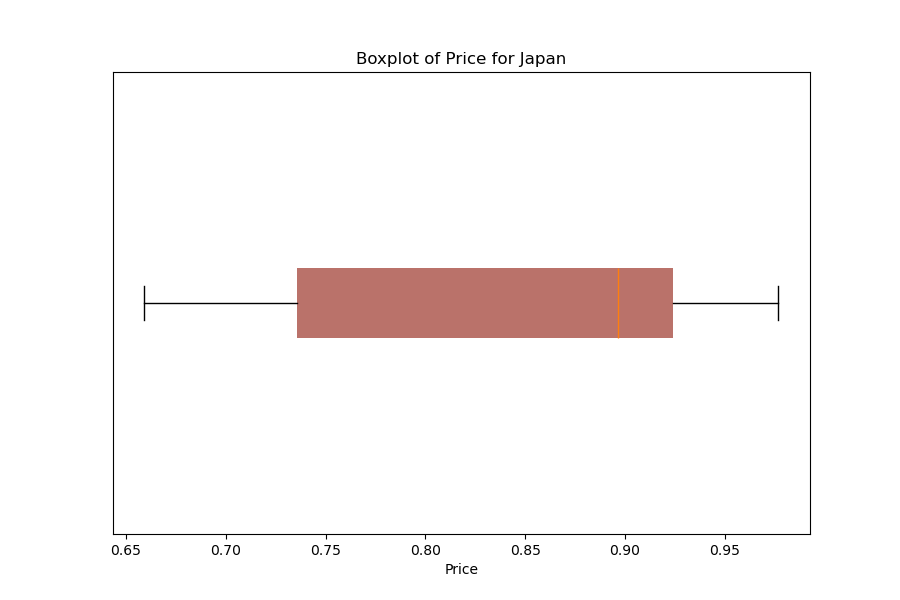
\includegraphics[width=1\textwidth]{bibliography/Figure/BoxPlot_Japan.png}
% %     \caption{Japan Currency Rate's boxplot}
% %     \label{fig:1}
% %     \end{minipage}
% %     \hfill
% %     \begin{minipage}{0.23\textwidth}
% %     \centering
% %     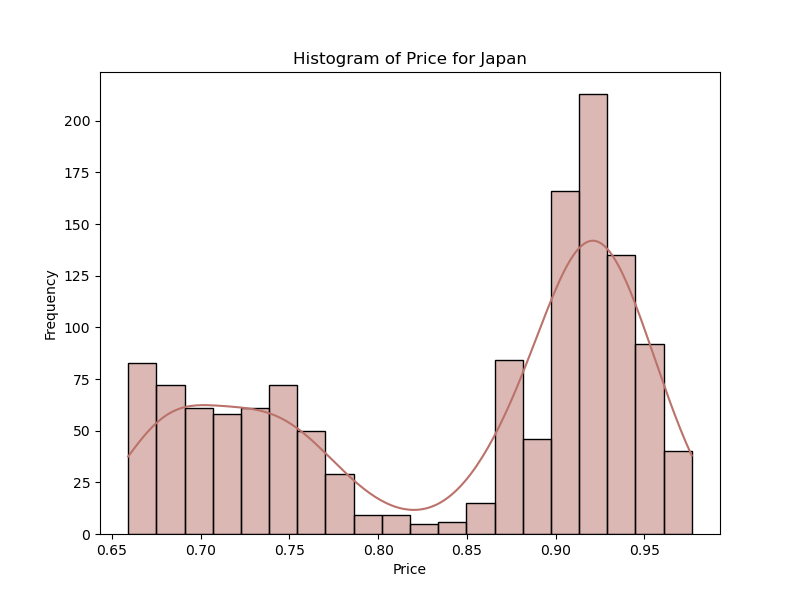
\includegraphics[width=1\textwidth]{bibliography/Figure/Histogram_Price_Japan.png}
% %     \caption{Japan Currency Rate's histogram}
% %     \label{fig:2}
% %     \end{minipage}
% % \end{figure}

% % \begin{figure}[!htbp]
% %     \centering
% %     \begin{minipage}{0.23\textwidth}
% %     \centering
% %     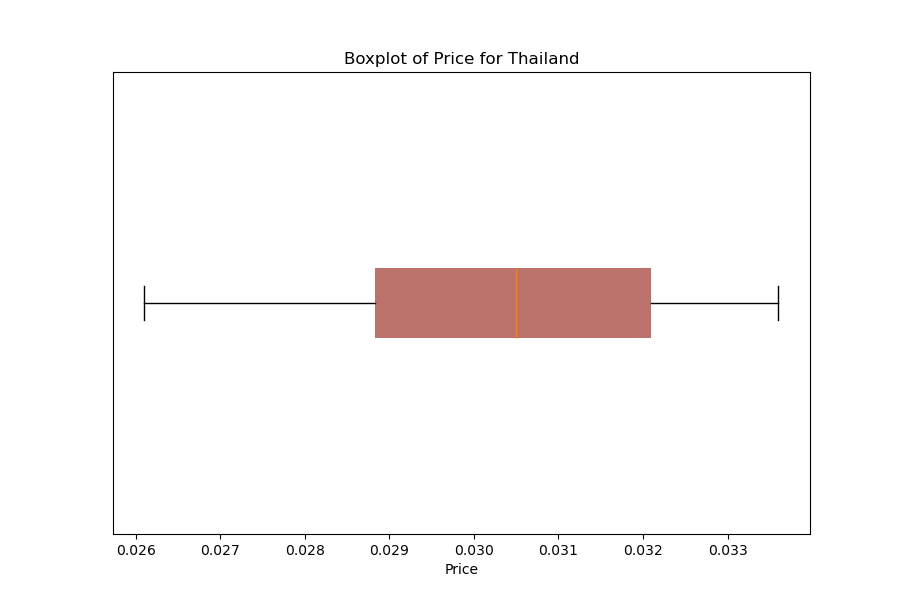
\includegraphics[width=1\textwidth]{bibliography/Figure/BoxPlot_Thailand.png}

% %     \caption{Thailand Currency Rate's boxplot}
% %     \label{fig:1}
% %     \end{minipage}
% %     \hfill
% %     \begin{minipage}{0.23\textwidth}
% %     \centering
% %     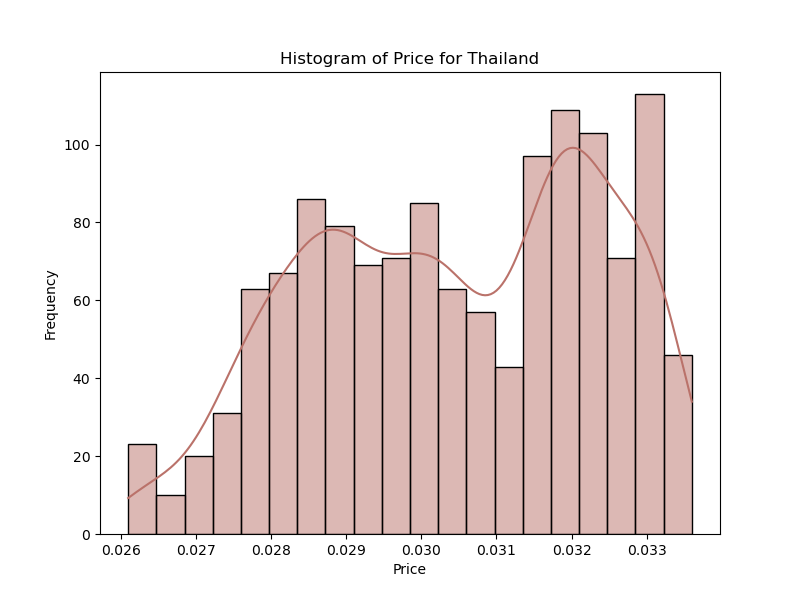
\includegraphics[width=1\textwidth]{bibliography/Figure/Histogram_Price_Thai.png}
% %     \caption{Thailand Currency Rate's histogram}
% %     \label{fig:2}
% %     \end{minipage}
% % \end{figure}

% % \begin{figure}[!htbp]
% %     \centering
% %     \begin{minipage}{0.23\textwidth}
% %     \centering
% %     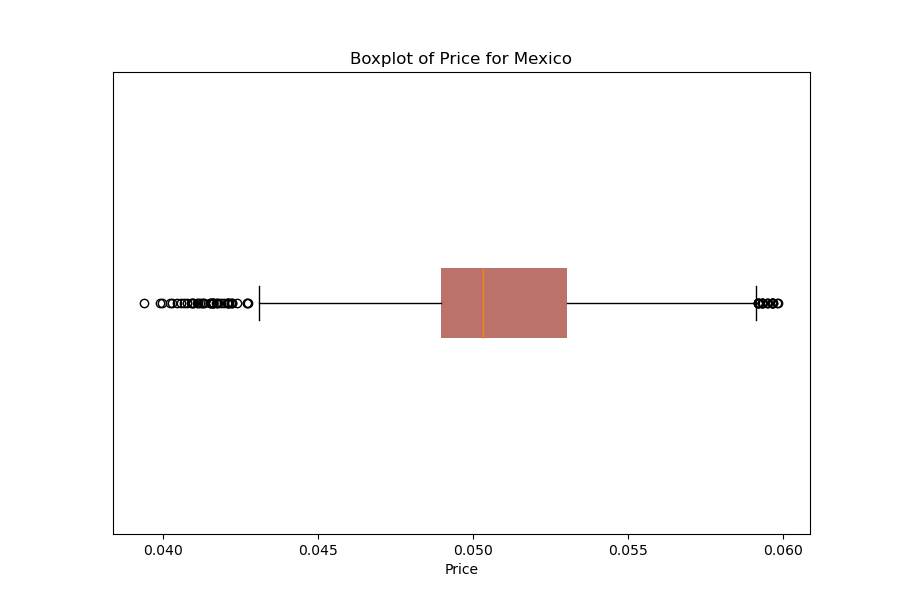
\includegraphics[width=1\textwidth]{bibliography/Figure/BoxPlot_Mexico.png}
% %     \caption{Mexico Currency Rate's boxplot}
% %     \label{fig:1}
% %     \end{minipage}
% %     \hfill
% %     \begin{minipage}{0.23\textwidth}
% %     \centering
% %     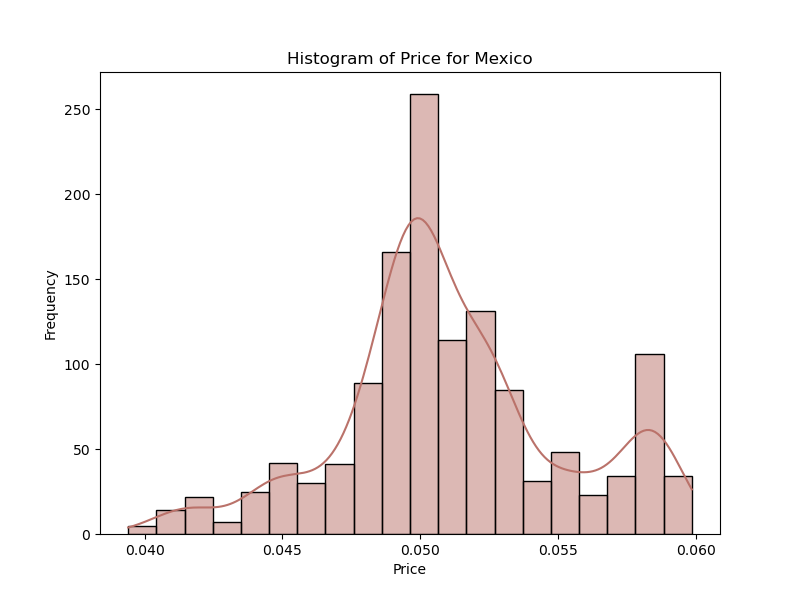
\includegraphics[width=1\textwidth]{bibliography/Figure/Histogram_Price_Mexico.png}
% %     \caption{Mexico Currency Rate's histogram}
% %     \label{fig:2}
% %     \end{minipage}
% % \end{figure}

% % \begin{table}[!htbp]
% %     \centering
% %     \caption{Japan, Thai, Mexico’s Descriptive Statistics}
% %   \begin{tabular}{|>{\columncolor{red!20}}c|c|c|c|}
% %       \hline
% %        \rowcolor{red!20} & Nhật Bản& Thái Lan& Mexico\\ \hline
% %        Count & 1306
% %   & 1306
% %   & 1306
% %   \\ \hline
% %        Mean & 0.840819
% %   & 0.030443
% %   & 0.051057
% %   \\ \hline
% %        Std & 0.659100
% %   & 0.026100
% %   & 0.039400
% %   \\ \hline
% %        Min & 0.735825
% %   & 0.028825
% %   & 0.048962
% %   \\ \hline
% %        25\% & 0.896600
% %   & 0.030500
% %   & 0.050330
% %   \\ \hline
% %        50\% & 0.924025
% %   & 0.032100
% %   & 0.053050
% %   \\ \hline
% %        75\% & 0.976800
% %   & 0.033600
% %   & 0.059860
% %   \\ \hline
% %        Max & 0.102068& 0.001906& 0.004094\\ \hline
% %   \end{tabular}
% %   \end{table}

% \FloatBarrier
% \section{Phương pháp}
% \label{sec:Phương pháp}

%     \subsection{Linear Regression}
%     Linear Regression, hay hồi quy tuyến tính, là một phương pháp thống kê được sử dụng để mô hình hóa mối quan hệ giữa một biến phụ thuộc và một hoặc nhiều biến độc lập. Mục tiêu của nó là tìm ra đường thẳng tốt nhất mô tả mối quan hệ này thông qua việc tối thiểu hóa tổng bình phương sai số giữa giá trị dự đoán và giá trị thực tế. Công thức của hồi quy tuyến tính có thể được biểu diễn như sau: \\
%     Đối với một biến độc lập:
%     \[y = \beta_0 + \beta_1 x + \epsilon\]
%         Trong đó: \\
%         \(y\): biến phụ thuộc \\
%         \(\beta_0\): hệ số chặn (intercept) \\
%         \(x\): biến độc lập (biến dự đoán)
%         \(\beta_1\): hệ số hồi quy cho biến độc lập
%         \(epsilon\): sai số ngẫu nhiên \\
%     Đối với nhiều biến độc lập:
%     \[y = \beta_0 + \beta_1 x_1 + \beta_2 x_2 + ... + \beta_n x_n +\epsilon\]
%         Trong đó: \\
%         \(y\): biến phụ thuộc \\
%         \(x_1,x_2,...,x_n\): là các biến độc lập \\
%         \(\beta_0\): hệ số chặn (intercept) \\
%         \(\beta_1,\beta_2,...,\beta_n\): hệ số hồi quy cho mỗi biến độc lập \\
%         \(\epsilon\): sai số ngẫu nhiên \\
%         Trong lĩnh vực tiền tệ, Linear Regression được sử dụng để dự đoán tỷ giá hối đoái, phân tích mối quan hệ giữa các yếu tố kinh tế và tỷ giá, dự báo biến động thị trường tài chính, và xác định các yếu tố ảnh hưởng đến giá và biến động của tiền tệ. 
%         % Tuy nhiên, Linear Regression có những hạn chế cơ bản như:
%         % \begin{itemize}
%         %                 \item Giả định Tuyến tính: Mô hình này giả định mối quan hệ tuyến tính giữa các biến độc lập và biến phụ thuộc, điều này không phải lúc nào cũng đúng trong thực tế.
%         %                 \item Nhạy cảm với Ngoại lệ: Hồi quy Tuyến tính rất nhạy cảm với các giá trị ngoại lệ (outliers), có thể ảnh hưởng đến độ chính xác của mô hình.
%         %                 \item Không xử lý tốt Dữ liệu Phi tuyến: Khi dữ liệu có mối quan hệ phi tuyến, mô hình Hồi quy Tuyến tính sẽ không phù hợp và cần phải sử dụng các mô hình phức tạp hơn.
%         %                 \item Giả định Độc lập: Mô hình này cũng giả định rằng các biến độc lập không tương quan với nhau, điều này có thể không đúng trong nhiều trường hợp thực tế.  \end{itemize}
%     \subsection{FFT (Fast Fourier Transform)}
%     Fast Fourier Transform (FFT) là một thuật toán được sử dụng để tính biến đổi Fourier rời rạc (DFT) và nghịch đảo của nó một cách hiệu quả. Nó chuyển đổi tín hiệu từ biểu diễn miền thời gian sang miền tần số, cho phép phát hiện các chu kỳ và mẫu lặp lại trong dữ liệu. 
    
%     Thuật toán FFT tính toán DFT của chuỗi bằng cách sử dụng phương pháp chia để trị dựa trên các cơ sở phức của đơn vị. DFT của một chuỗi [X] có độ dài N được định nghĩa theo công thức:
    
%     \[
%     X[k] = \sum_{n=0}^{N-1} x[n] e^{-i \frac{2\pi nk}{N}}
%     \]
    
%     \begin{itemize}
%         \item \(X[k]\): đại diện cho biểu diễn miền tần số.
%         \item \(x[n]\): là chuỗi dữ liệu miền thời gian.
%         \item \(N\): là độ dài của chuỗi miền thời gian.
%         \item \(e^{-i \frac{2\pi nk}{N}}\): là đơn vị phức thuần túy được sử dụng trong quá trình biến đổi.
%     \end{itemize}
    
%     Mục tiêu chính của FFT là phân tích và hiểu các thành phần tần số có trong tín hiệu, cho phép các ứng dụng xử lý tín hiệu, truyền thông, xử lý âm thanh, xử lý hình ảnh, v.v. FFT trong dự báo hối đoái có lợi thế về tính hiệu quả và tốc độ xử lý. Tuy nhiên, giả định về tính chu kỳ của tín hiệu có thể gây nhiễu và hạn chế độ phân giải tần số.
    
%     \subsection{ARIMA (Autoregressive Integrated Moving Average)}
% ARIMA model là viết tắt của cụm từ Autoregressive Integrated Moving Average. Mô hình sẽ biểu diễn phương trình hồi quy tuyến tính đa biến (multiple linear regression) của các biến đầu vào (còn gọi là biến phụ thuộc trong thống kê) là 2 thành phần chính: 

% \textbf{Auto regression:} Kí hiệu là AR. Đây là thành phần tự hồi quy bao gồm tập hợp các độ trễ của biến hiện tại. Độ trễ bậc \(p\) chính là giá trị lùi về quá khứ \(p\) bước thời gian của chuỗi. Độ trễ dài hoặc ngắn trong quá trình AR phụ thuộc vào tham số trễ \(p\). Cụ thể, quá trình AR(\(p\)) của chuỗi \(x_t\) được biểu diễn như bên dưới:
% \[
% AR(p) = \phi_0 + \phi_1 x_{t-1} + \phi_2 x_{t-2} + \cdots + \phi_p x_{t-p}
% \]

% \textbf{Moving average:} Quá trình trung bình trượt được hiểu là quá trình dịch chuyển hoặc thay đổi giá trị trung bình của chuỗi theo thời gian. Do chuỗi của chúng ta được giả định là dừng nên quá trình thay đổi trung bình dường như là một chuỗi nhiễu trắng. Quá trình moving average sẽ tìm mối liên hệ về mặt tuyến tính giữa các phần tử ngẫu nhiên \(\epsilon_t\) (stochastic term). Chuỗi này phải là một chuỗi nhiễu trắng thỏa mãn các tính chất:
% \[ 
% \begin{cases}
% E(\epsilon_t) = 0 \\
% \sigma(\epsilon_t) = \alpha \\
% p(\epsilon_t, \epsilon_{t-s}) = 0
% \end{cases}
% \]

% ARIMA tích hợp hai quy trình: quy trình tự hồi quy bậc \(p\) – AR(\(p\)) và quy trình trung bình trượt bậc \(q\) – MA(\(q\)). Mặt khác, cần phải sử dụng phân tích tích phân sai I(\(d\)) (hay còn gọi là toán tử tự động) để làm cho chuỗi thời gian dừng lại.

% \textbf{Mô hình hồi quy tự động (AR) (p):}
% \[
% Y_t = \alpha + \theta_1 \varepsilon_{t-1} + \theta_2 \varepsilon_{t-2} + \cdots + \theta_p \varepsilon_{t-p} + \varepsilon_{t}
% \]
% Trong đó: \\
% \(\alpha\) là một hằng số. \\
% \(Y_{t-1},\ldots,Y_{t-p}\) là độ trễ của chuỗi. \\
% \(\varepsilon_{t}\) là nhiễu trắng. 

% \textbf{Mô hình trung bình di chuyển tích hợp hồi quy tự động (ARIMA) (p,q,d):}
% \[
% \nabla Y_t = \alpha + \beta_1 \nabla Y_{t-1} + \cdots + \beta_p \nabla Y_{t-p} + \theta_1 \varepsilon_{t-1} + \theta_q \varepsilon_{t-q} + \varepsilon_t
% \]

% Mô hình ARIMA không phải là mô hình dự báo hoàn hảo cho bất kỳ chuỗi thời gian nào và chỉ hoạt động tốt nhất nếu dữ liệu phụ thuộc vào thời gian và dự báo thuộc loại thời gian, dữ liệu ngẫu nhiên thường ít hoạt động với mô hình ARIMA.

%     \subsection{RNN (Recurrent Neural Network)}

%     Là một lớp mạng nơ-ron có tính năng đặc biệt trong 
%     việc mô hình hóa dữ liệu chuỗi và chuỗi thời gian. 
%     RNN hoạt động bằng cách duy trì một trạng thái ẩn \( h(t) \)
%     tại mỗi bước thời gian (t) để lưu lại thông tin từ các bước 
%     trước đó và sử dụng thông tin đó để dự đoán đầu ra tại 
%     mỗi bước thời gian tiếp theo.
    
%         \begin{figure}[!htbp]
%             \centering
%             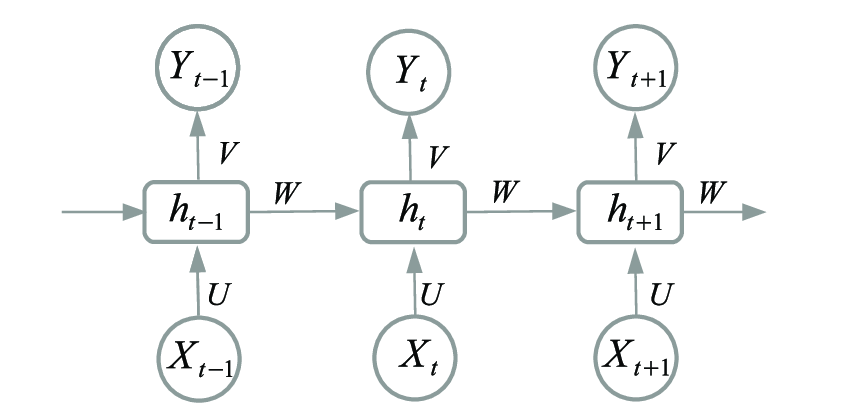
\includegraphics[width=0.4\textwidth]{bibliography/Figure/RNN model.png}
%             \caption{Mô hình RNN}
%             \label{fig:rnn_model}
%         \end{figure}
%         \[
%         h_t = \sigma (W^{hh} h_{t-1} + W^{hx} x_t)
%         \]
%         Ký hiệu:
%         \begin{itemize}
%             \item \( h(t) \): trạng thái mới
%             \item \( h(t-1) \): trạng thái cũ
%             \item \( x(t) \): vector đầu vào tại thời điểm t
%         \end{itemize}

%         Mô hình RNN với hàm kích hoạt sigmoid và đầu ra SoftMax:

%                 \[
%                 y_t = \text{softmax}(W^{(s)} h_t)
%                 \]

%     \subsection{GRU (Gated Recurrent Unit)}

%     Thuật toán GRU (Gated Recurrent Unit) là một kiến trúc mạng nơ-ron hồi quy được thiết kế để giải quyết vấn đề biến mất gradient và cải thiện hiệu suất so với mạng nơ-ron hồi quy truyền thống (RNN). GRU giống như LSTM nhưng có cấu trúc đơn giản hơn, chỉ bao gồm hai cổng chính: cổng cập nhật (update gate) và cổng reset (reset gate).
    
%     \begin{figure}[h]
%         \centering
%     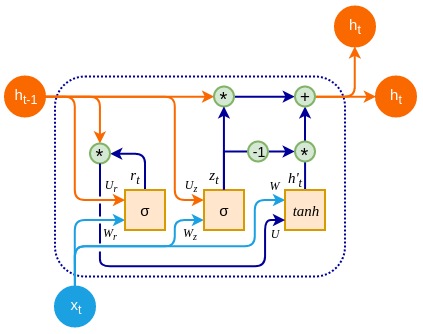
\includegraphics[width=0.5
%     \textwidth]{BichHao/GRU.png}
%         \caption{Mô hình GRU}
%         \label{fig:example}
%     \end{figure}

%     Cách hoạt động của GRU như sau:
%     \begin{itemize}
%         \item Cổng Đặt Lại: Xác định xem liệu nên quên thông tin từ quá khứ bằng cách đặt lại cổng, một neuron sigmoid. Nếu cổng đặt lại đưa ra giá trị gần 0, nó sẽ bỏ qua thông tin từ quá khứ.
%         \item Cổng Cập Nhật: Xác định thông tin mới nào sẽ được lưu trữ trong trạng thái ẩn mới. Điều này được thực hiện thông qua cổng cập nhật, một neuron sigmoid khác, quyết định xem thông tin mới nên được lưu trữ hoàn toàn từ đầu vào hiện tại, hay chỉ một phần kết hợp với thông tin từ quá khứ.
%         \item Trạng Thái Ẩn Mới: Cuối cùng, GRU tính toán trạng thái ẩn mới dựa trên cổng đặt lại, cổng cập nhật và đầu vào hiện tại. Trạng thái ẩn mới này là kết hợp của trạng thái ẩn trước đó và thông tin mới từ đầu vào, được điều chỉnh bởi các cổng.
%         \begin{figure}
%         \centering
%         \label{fig:example}
%     \end{figure}
%     \end{itemize}
    
%     \textbf{Step by step to calculation}
    
%     Tại bước thời gian \( t \) với biến đầu vào \( x_t \) \( \in R^n \times d \) (số lượng mẫu: \( n \), số lượng đầu vào: \( d \)) và trạng thái ẩn gần nhất \( h_{t-1} \) \( \in R^n \times h \) (số lượng trạng thái ẩn: \( h \)), cổng đặt lại \( r_t \) \( \in R^n \times h \) và cổng cập nhật \( z_t \) \( \in R^n \times h \) được tính bằng các công thức sau:
%     \[
%     r_t = \sigma(wx_r \cdot x_t + wh_r \cdot h_{t-1} + b_r)
%     \]
%     \[
%     z_t = \sigma(wx_z \cdot x_t + wh_z \cdot h_{t-1} + b_z)
%     \]
    
%     Ở đây, \( wx_r \), \( wh_z \) \( \in R^d \times h \) và \( wx_r \), \( wh_z \) \( \in R^h \times h \) là các tham số trọng số, và \( b_r \), \( b_z \) \( \in R^{1 \times h} \) là các thuật ngữ độ lệch.
    
%     Cổng đặt lại được tính bằng cách xem xét cả trạng thái ẩn trước đó và đầu vào hiện tại, sau đó quyết định các dữ liệu nào trong quá khứ nên bị quên. Tính toán được đạt được thông qua việc cộng trạng thái ẩn trước đó với đầu vào hiện tại sau khi chúng được nhân với trọng số tương ứng của chúng và cộng một thuật ngữ độ lệch, sau đó đi qua hàm chuyển đổi sigmoid. Hàm này biến đổi giá trị thành khoảng từ 0 đến 1, cho phép cổng xác định và lọc thông tin quan trọng và không quan trọng cho các trạng thái tiếp theo, qua biểu thức:
    
%     \[
%     r(t) = (wx_r \cdot x_t \times wh_r \cdot h_{t-1} + b_r)
%     \]
    
%     Khi toàn bộ mạng được đào tạo thông qua lan truyền ngược, các trọng số trong phương trình sẽ được cập nhật sao cho vector sẽ học cách chỉ giữ lại các thông tin hữu ích. Các trạng thái ẩn ban đầu \( h_{t-1} \) sẽ thực hiện phép nhân thông minh với vector đặt lại và sau đó nhân với trọng số của khả năng huấn luyện. Đồng thời, đầu vào hiện tại \( x_t \) sẽ được nhân với trọng số. Cuối cùng, hàm tanh phi tuyến tính sẽ được áp dụng cho kết quả cuối cùng để thu được \( h_t \) theo công thức dưới đây:
    
%     \[
%     h_t = \tanh(w \cdot [r(t) \times h_{t-1}] + wx_t)
%     \]
    
%     Cổng cập nhật có công thức tương tự như cổng đặt lại, nhưng các trọng số nhân khác nhau, cho phép cổng thực hiện một mục đích cụ thể của nó. Cổng cập nhật hoạt động dựa trên phương trình sau:
    
%     \[
%     z(t) = (wx_z \cdot x_t \times wh_z \cdot h_{t-1} + b_z)
%     \]
    
%     Tích hợp hoạt động, cổng cập nhật kiểm soát lượng thông tin từ trạng thái ẩn trước đó sẽ chuyển sang trạng thái ẩn hiện tại và xác định mức độ giống nhau giữa trạng thái mới \( h_t \) và trạng thái cũ \( h_{t-1} \), cũng như mức trạng thái ẩn tiềm năng. Áp dụng phương trình cập nhật cuối cùng:
    
%     \[
%     h(t) = z_t \times h_{t-1} + (1 - z_t) \times h_t
%     \]
    
%     GRU là mô hình được áp dụng đặc biệt trong dự báo chuỗi thời gian. Đây là phương pháp mang một kiến trúc tương đối mới khi so sánh với với một số phương pháp đã được áp dụng rộng rãi như LSTM thì GRU cho hiệu xuất nhanh hơn do GRU có cổng ít hơn LSTM một cổng vì lý do này GRU tiết kiệm chi phí và thực hiện khối lượng tính toán ít hơn.
    
%     % GRU có thể hiệu quả hơn LSTM trong một số trường hợp do cấu trúc đơn giản hơn và ít tham số hơn, làm cho việc huấn luyện nhanh hơn và giảm thiểu nguy cơ quá mức học (overfitting). Tuy nhiên, cả hai kiến trúc đều có thể được sử dụng cho các nhiệm vụ dự đoán và phân tích dữ liệu chuỗi thời gian và ngôn ngữ tự nhiên.
    
%     \subsection{LSTM (Long Short-Term Memory)}
% LSTM là một loại mạng nơ-ron hồi quy (recurrent neural network - RNN) được sử dụng rộng rãi trong việc xử lý và dự báo chuỗi thời gian, cũng như trong các bài toán liên quan đến ngôn ngữ tự nhiên và xử lý dữ liệu tuần tự.

% LSTM là một kiến trúc mạng nơ-ron đặc biệt thiết kế để xử lý vấn đề biến mất gradient trong việc huấn luyện mạng nơ-ron hồi quy (RNN). RNN thường gặp vấn đề khi cố gắng học các phụ thuộc xa trong dữ liệu chuỗi, khiến cho nó khó học được các mối quan hệ dài hạn trong dữ liệu chuỗi thời gian. LSTM giải quyết vấn đề này bằng cách sử dụng cơ chế cập nhật bộ nhớ, cho phép nó ghi nhớ thông tin quan trọng từ quá khứ và sử dụng nó trong tương lai.

% Cách thức hoạt động của LSTM như sau: 
% % \begin{figure}[h!]
% %     \centering
% %     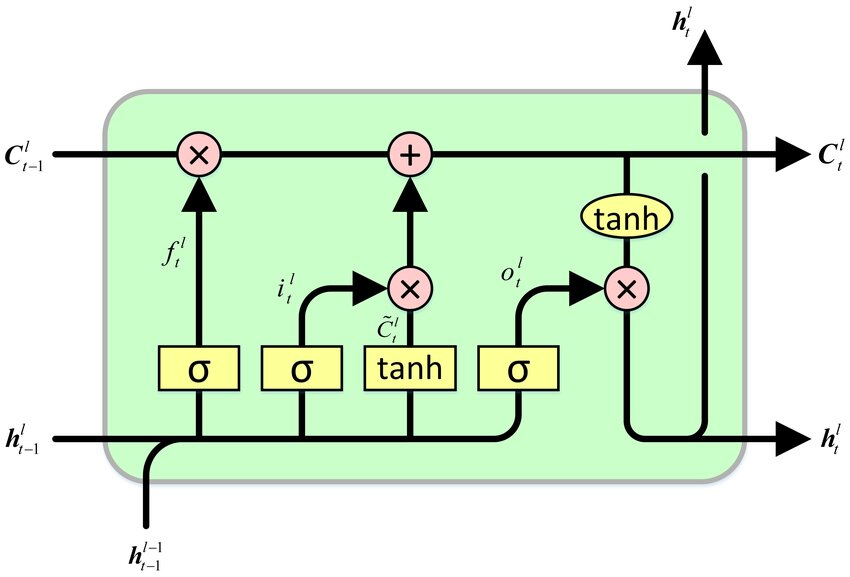
\includegraphics[width=0.3\textwidth]{BichHao/LSTM.png}
% %     \caption{Cách hoạt động LSTM}
% %     \label{fig:your_label}
% % \end{figure}
%                 \begin{itemize}
%                     \item Cổng quên (Forget gate): Đầu tiên, LSTM quyết định thông tin nào từ bộ nhớ trước đó sẽ được quên đi. Điều này được thực hiện bằng cách sử dụng một cổng quên, một mạng nơ-ron có giá trị từ 0 đến 1, mà giá trị 1 tương ứng với việc giữ lại tất cả thông tin và giá trị 0 tương ứng với việc quên hết thông tin.
%                     \item Cổng đầu vào (Input gate): LSTM tiếp tục bằng việc quyết định thông tin mới nào sẽ được lưu trữ trong bộ nhớ. Điều này được thực hiện thông qua cổng đầu vào, một mạng nơ-ron sigmoid và một lớp tanh. Cổng này quyết định giá trị mới nào sẽ được thêm vào bộ nhớ.
%                     \item Cổng đầu ra (Output gate):Cuối cùng, LSTM quyết định thông tin nào từ bộ nhớ sẽ được đưa ra dưới dạng đầu ra của mô hình. Điều này được thực hiện thông qua cổng đầu ra, một mạng nơ-ron sigmoid và một lớp tanh, tương tự như cổng đầu vào.
%                     \item Cell State (Trạng Thái Bộ Nhớ): LSTM sử dụng một cell state (trạng thái bộ nhớ) để lưu trữ và truyền tải thông tin qua các bước thời gian. Trạng thái này được cập nhật thông qua các cổng quên và cổng đầu vào, giúp LSTM ghi nhớ thông tin quan trọng trong dữ liệu chuỗi.
%                 \end{itemize}
                
% Nhờ vào các cổng này và trạng thái bộ nhớ, LSTM có khả năng học và ghi nhớ các phụ thuộc xa trong dữ liệu chuỗi, giúp nó hiệu quả trong việc dự đoán và phân tích các dữ liệu chuỗi thời gian và ngôn ngữ tự nhiên.

% LSTM đã chứng tỏ hiệu suất tốt trong việc mô hình hóa và dự báo các chuỗi thời gian phức tạp, cũng như trong các bài toán xử lý ngôn ngữ tự nhiên như dịch máy, sinh văn bản và nhận diện giọng nói. Nó đã trở thành một công cụ quan trọng trong lĩnh vực trí tuệ nhân tạo và học máy.

% \subsection{TBATS}
% TBATS là một khung dự báo được giới thiệu để dự báo chuỗi thời gian với các mẫu mùa phức tạp như nhiều chu kỳ mùa, mùa tần số cao, mùa không nguyên và hiệu ứng lịch kép. Tên TBATS là viết tắt của:
% \begin{itemize}
%     \item T: Trigonometric seasonality (mùa vụ lượng giác)
%     \item B: Box-Cox transformation (biến đổi Box-Cox)
%     \item A: ARMA errors (sai số ARMA)
%     \item T: Trend (xu hướng)
%     \item S: Seasonal components (các thành phần mùa vụ)
% \end{itemize}

% Cách hoạt động của TBATS
% \begin{itemize}
%     \item Chuẩn bị và Biến đổi Dữ liệu Box-Cox Transformation: Bước này ổn định phương sai và làm cho dữ liệu có phân phối chuẩn hơn. Biến đổi được định nghĩa như sau:
%         \[
%         y_t^{(\omega)} =
%         \begin{cases}
%         \frac{y_t^{\omega} - 1}{\omega}, & \text{nếu } \omega \neq 0 \\
%         \log(y_t), & \text{nếu } \omega = 0
%         \end{cases}
%         \]

%     \item Biểu diễn Không gian Trạng thái: Mô hình TBATS được hình thành dưới dạng mô hình không gian trạng thái bao gồm mức độ, xu hướng và nhiều thành phần mùa:
%         \[
%         y_t^{(\omega)} = \ell_{t-1} + \phi b_{t-1} + \sum_{i=1}^{T} s_{t-m_i}^{(i)} + d_t
%         \]
%     Trong đó:
%         \begin{itemize}
%             \item $\ell_t$ là thành phần mức độ
%             \item $b_t$ là thành phần xu hướng
%             \item $s_{t}^{(i)}$ là các thành phần mùa với chu kỳ $m_i$
%             \item $d_t$ là sai số
%         \end{itemize}

%     \item Thành phần của mô hình: Các thành phần mức độ và xu hướng được cập nhật như sau:
%         \[
%         \ell_t = \ell_{t-1} + \phi b_{t-1} + \alpha d_t
%         \]

%         \[
%         b_t = (1 - \phi)b + \phi b_{t-1} + \beta d_t
%         \]
%     Trong đó: $\phi$ là tham số giảm dần, $\alpha$ và $\beta$ là các tham số làm trơn.

%     \item Thành phần Mùa: mỗi thành phần mùa được mô hình hóa bằng các hàm lượng giác:
%         \[
%         s_t^{(i)} = \sum_{j=1}^{k_i} s_{j,t}^{(i)}
%         \]

%         \[
%         s_{j,t}^{(i)} = s_{j,t-1}^{(i)} \cos(\lambda_j^{(i)}) + s_{j,t-1}^{(i)*} \sin(\lambda_j^{(i)}) + \gamma_1^{(i)} d_t
%         \]

%         \[
%         s_{j,t}^{(i)*} = -s_{j,t-1}^{(i)} \sin(\lambda_j^{(i)}) + s_{j,t-1}^{(i)*} \cos(\lambda_j^{(i)}) + \gamma_2^{(i)} d_t
%         \]
%         Trong đó: \(\lambda_j(i) = \frac{2 \pi j}{m_i}\) và \(\gamma_1(i)\) và \(\gamma_2(i)\) là các tham số làm trơn.
%     \item Thành phần sai số và ARMA: thành phần sai số $d_t$ có thể tuân theo một quá trình ARMA để tính đến tự tương quan trong phần dư:
%         \[
%         d_t = \sum_{i=1}^{p} \varphi_i d_{t-i} + \sum_{j=1}^{q} \theta_j \epsilon_{t-j} + \epsilon_t
%         \]
%         Trong đó $\varphi_i$ và $\theta_i$ là các tham số ARMA, và $\epsilon_t$ là nhiễu trắng Gaussian.
%     \item Lựa chọn Mô hình: Tiêu chí Thông tin Akaike (AIC) thường được sử dụng để chọn mô hình tốt nhất trong các cấu hình TBATS khác nhau. Mô hình có AIC thấp nhất được chọn.

% \end{itemize}


% \subsection{Boosting Model}
% Boosting là một kỹ thuật mô hình hóa Ensemble xây dựng một bộ phân loại mạnh mẽ từ một số lượng bộ phân loại yếu. Nó được thực hiện bằng cách xây dựng một mô hình bằng cách sử dụng các mô hình yếu theo chuỗi. Đầu tiên, một mô hình được xây dựng từ dữ liệu huấn luyện. Sau đó, mô hình thứ hai được xây dựng để sửa các lỗi có mặt trong mô hình đầu tiên. Thủ tục này được tiếp tục và các mô hình được thêm vào cho đến khi hoặc toàn bộ dữ liệu huấn luyện được dự đoán đúng hoặc số lượng mô hình tối đa được thêm vào.
% % \begin{figure}[h!]
% %     \centering
% %     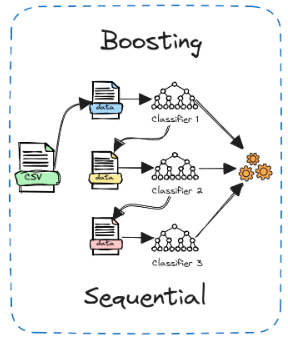
\includegraphics[width=0.3\textwidth]{BichHao/Boosting1.png}
% %     \caption{Cách hoạt động của Boosting}
% %     \label{fig:your_label}
% % \end{figure}

% Có một số loại thuật toán Boosting, một số mô hình nổi tiếng và hữu ích nhất là:
% \begin{itemize}
%     \item Gradient Boosting
%     \item XGBoost
%     \item AdaBoost
%     \item CatBoost
% \end{itemize}

% % Mô hình Ensemble là một kỹ thuật kết hợp nhiều mô hình học máy để cải thiện hiệu suất dự đoán tổng thể. Ý tưởng cơ bản là một nhóm các Model (Tập dữ liệu được chọn để trải qua training với thuật toán cụ thể) có tính dự đoán yếu có thể hợp nhất để tạo thành một Model có tính dự đoán mạnh mẽ.

% % Một mô hình Ensemble thường bao gồm hai bước:
% % \begin{enumerate}
% %     \item Nhiều Model học máy được huấn luyện độc lập.
% %     \item Dự đoán của chúng được tổng hợp theo một cách nào đó, như bằng cách bỏ phiếu, trung bình hoặc trọng số. Ensemble này sau đó được sử dụng để đưa ra dự đoán tổng thể.
% % \end{enumerate}

% % Ensemble thường cho kết quả tốt hơn vì các mô hình khác nhau bổ sung cho nhau và vượt qua các điểm yếu cá nhân của họ. Chúng cũng giảm phương sai và over-fitting.
% % \begin{figure}[h!]
% %     \centering
% %     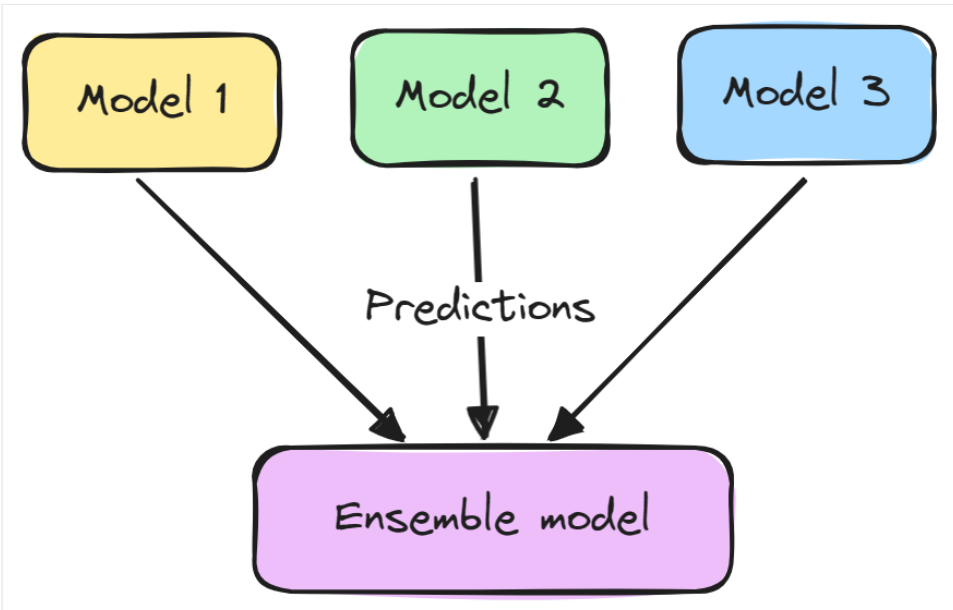
\includegraphics[width=0.3\textwidth]{BichHao/Boosting2.png}
% %     \caption{Cách thực nghiệm Ensemble với Boosting}
% %     \label{fig:your_label}
% % \end{figure}

% Quá trình huấn luyện của mô hình Boosting có thể được mô tả như sau:
% \begin{enumerate}
%     \item Khởi tạo tập dữ liệu và gán trọng số bằng nhau cho mỗi điểm dữ liệu. Bắt đầu với việc gán cho mỗi mẫu trong tập dữ liệu một trọng số bằng nhau.
%     \item Cung cấp tập dữ liệu này làm đầu vào cho mô hình và xác định các điểm dữ liệu bị phân loại sai. Mô hình được huấn luyện trên tập dữ liệu hiện tại và sử dụng để dự đoán. Các điểm dữ liệu được xác định sai lầm sẽ được ghi nhận.
%     \item Tăng trọng số cho các điểm dữ liệu bị phân loại sai. Sau khi xác định các điểm dữ liệu bị phân loại sai, ta tăng trọng số của chúng. Điều này làm cho các điểm dữ liệu này có ảnh hưởng lớn hơn đến quá trình huấn luyện tiếp theo.
%     \item Kiểm tra xem có đạt được kết quả yêu cầu không. Kiểm tra điều kiện dừng nếu đạt được kết quả yêu cầu, chẳng hạn như số lượng lần lặp đã đủ hoặc độ chính xác đã đạt một ngưỡng nhất định.
%     \item Quay lại Bước 2 nếu kết quả chưa đạt được. Nếu không đạt được kết quả yêu cầu, tiếp tục quá trình huấn luyện bằng cách quay lại Bước 2 với tập dữ liệu được cập nhật với các trọng số mới.
%     \item Kết thúc quá trình huấn luyện. Khi đạt được kết quả yêu cầu, kết thúc quá trình huấn luyện và sử dụng mô hình Ensemble đã được tạo ra để dự đoán trên dữ liệu mới.
%     \begin{figure}[h!]
%     \centering
%     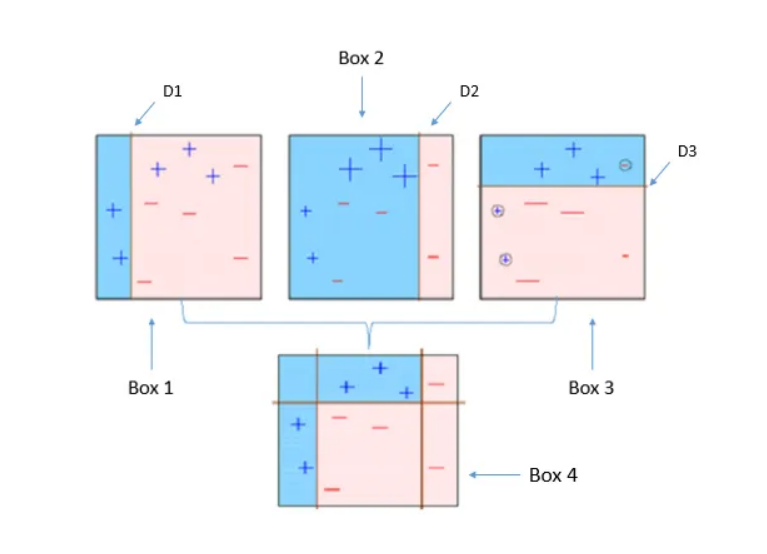
\includegraphics[width=0.5\textwidth]{BichHao/Boosting3.png}
%     \caption{Ví dụ thực nghiệm Boosting}
%     \label{fig:your_label}
% \end{figure}

% \end{enumerate}
% % Ví dụ cách Boosting Model hoạt động:
% % \begin{itemize}
% %     \item \textbf{Step 1}: Bắt đầu từ Box 1, gán các trọng số bằng nhau (được biểu thị bằng kích thước của các dấu hiệu) cho tất cả đầu vào và dự đoán "+" cho đầu vào ở vùng màu xanh và "-" cho đầu vào ở vùng màu đỏ, sử dụng gốc quyết định D1.
% %     \item \textbf{Step 2}: Trong lần lặp tiếp theo, Box 2, bạn có thể thấy trọng số của các dấu cộng được phân loại sai sẽ lớn hơn các đầu vào khác. Vì vậy, gốc quyết định D2 được chọn sao cho những quan sát này hiện được phân loại chính xác.
% %     \item \textbf{Step 3}: Trong lần lặp lại cuối cùng, Box 3 có 3 âm bản bị phân loại sai tại khu vực màu đỏ. Vì vậy gốc quyết định D3 được chọn để sửa lỗi đó bằng cách tiếp tục tăng trọng số của 3 âm này.
% %     \item \textbf{Step 4}: Cuối cùng, tổng hợp từ 3 kết quả dự đoán đưa ra một quy tắc mạnh và có độ chính xác cao được tạo ra bằng cách kết hợp các gốc quyết định yếu riêng lẻ.
% % \end{itemize}
% Với Boosting, các mô hình được huấn luyện tuần tự, với mỗi mô hình học từ các sai lầm của mô hình trước đó. Mỗi mô hình được tạo ra sau một vòng lặp đặc biệt để tối ưu hóa mục tiêu, thường là giảm thiểu lỗi dự đoán.

% Ngoài ra, trong Boosting, trọng số được gán cho mỗi điểm dữ liệu dựa trên độ chính xác của mô hình trước đó. Cụ thể, các điểm dữ liệu được phân loại sai bởi mô hình trước đó sẽ có trọng số cao hơn trong quá trình huấn luyện mô hình tiếp theo.

% Boosting thường kết hợp các dự đoán từ các mô hình khác nhau để tạo ra dự đoán tổng thể. Các mô hình này thường thuộc các loại khác nhau, có thể là Decision Tree (Cây quyết định), Regression (Hồi quy tuyến tính)...

% Mục tiêu chính của Boosting là giảm thiểu sai số cố định (bias) chứ không phải là giảm phương sai (variance). Sai số cố định (bias) đo lường mức độ chính xác của dự đoán so với giá trị thực tế. Khi sai số cố định cao, mô hình có xu hướng phân loại dự đoán sai hoặc không chính xác. Boosting tập trung vào việc giảm thiểu sai số cố định bằng cách tạo ra các mô hình tuần tự và học từ các sai lầm của các mô hình trước đó. Điều này giúp cải thiện tính chính xác và hiệu suất của mô hình.


%     \subsection{FEDformer}
%     FEDformer (Frequency Enhanced Decomposed Transformer) là một mô hình dự báo chuỗi thời gian dài hạn bằng cách kết hợp Transformer với phương pháp phân rã xu hướng mùa vụ (Seasonal-Trend Decomposition) để cải thiện khả năng dự báo
%         \begin{figure}[h]
%             \centering
%         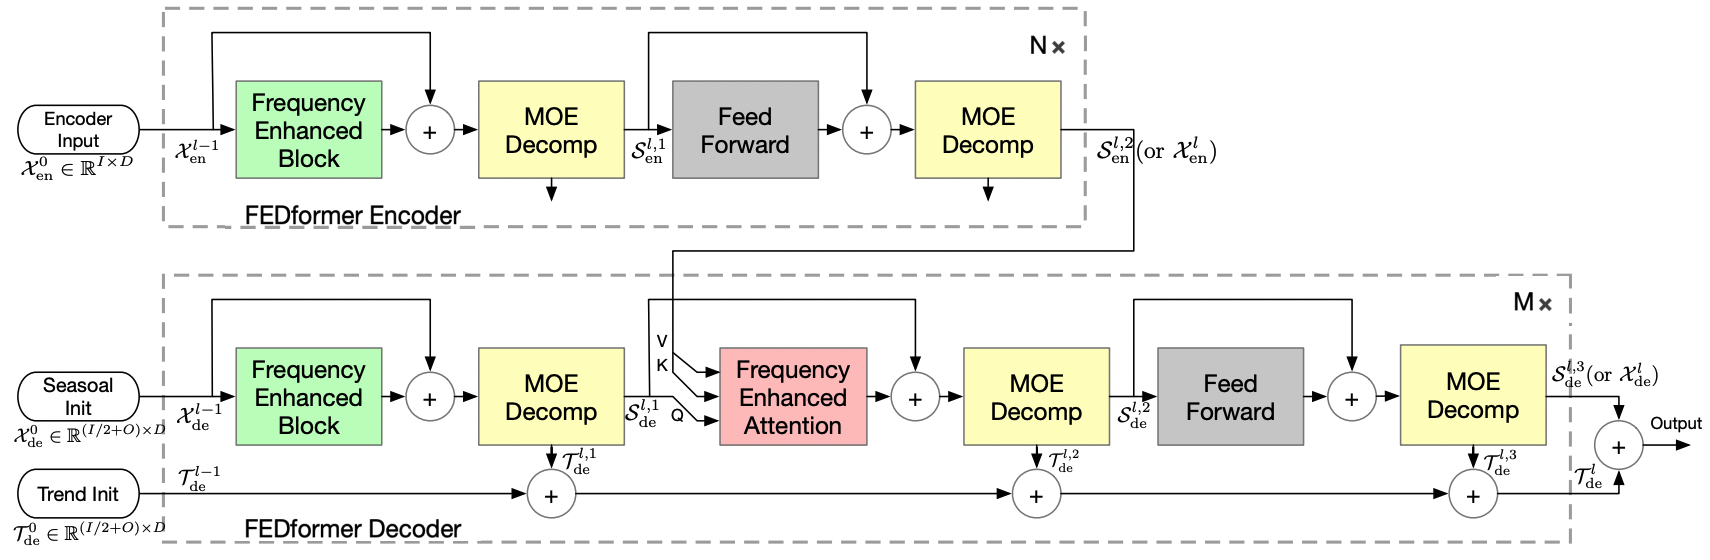
\includegraphics[width=0.5
%         \textwidth]{FEDFormer/FEDFormer.png}
%             \caption{Flow diagram of the FEDformer}
%             \label{fig:example}
%         \end{figure}
%         \paragraph{Tổng quan về mô hình FEDformer}
        
        
%         \paragraph*{1.FEDFormer Encoder}
        
%         \begin{enumerate}
%             \item \textbf{Encoder Input} ($X_{en}^0$):
%             \begin{itemize}
%                 \item Đầu vào của bộ mã hóa có kích thước $I \times D$.
%             \end{itemize}
            
%             \item \textbf{Frequency Enhanced Block (FEB)}:
%             \begin{itemize}
%                 \item Chuyển đổi đầu vào $X_{en}^{l-1}$ sang miền tần số bằng phép biến đổi Fourier (DFT).
%                 \item Xử lý các thành phần tần số và chuyển đổi ngược lại về miền thời gian (IDFT).
%             \end{itemize}
            
%             \item \textbf{MOE Decomp (Mixture of Experts Decomposition)}:
%             \begin{itemize}
%                 \item Sử dụng các bộ lọc trung bình để trích xuất và kết hợp các thành phần xu hướng và mùa vụ.
%             \end{itemize}
            
%             \item \textbf{Feed Forward}:
%             \begin{itemize}
%                 \item Lớp mạng nơ-ron tiến truyền giúp tăng cường khả năng biểu diễn của mô hình.
%             \end{itemize}
            
%             \item \textbf{Kết hợp}:
%             \begin{itemize}
%                 \item Kết quả từ các khối khác nhau được kết hợp lại bằng phép cộng.
%             \end{itemize}
            
%             \item \textbf{N lần lặp lại}:
%             \begin{itemize}
%                 \item Toàn bộ phần Encoder được lặp lại N lần để tăng cường khả năng học của mô hình.
%             \end{itemize}
%         \end{enumerate}
        
%         \paragraph*{2.FEDFormer Decoder}
        
%         \begin{enumerate}
%             \item \textbf{Seasonal Init} và \textbf{Trend Init}:
%             \begin{itemize}
%                 \item Khởi tạo các thành phần mùa vụ và xu hướng cho phần giải mã, có kích thước $(I/2 + O) \times D$.
%             \end{itemize}
            
%             \item \textbf{Frequency Enhanced Block (FEB)}:
%             \begin{itemize}
%                 \item Tương tự như phần mã hóa, chuyển đổi và xử lý đầu vào trong miền tần số.
%             \end{itemize}
            
%             \item \textbf{MOE Decomp}:
%             \begin{itemize}
%                 \item Tương tự như phần mã hóa, trích xuất và kết hợp các thành phần xu hướng và mùa vụ.
%             \end{itemize}
            
%             \item \textbf{Frequency Enhanced Attention (FEA)}:
%             \begin{itemize}
%                 \item Thực hiện attention trong miền tần số để tập trung vào các thành phần quan trọng.
%             \end{itemize}
            
%             \item \textbf{Feed Forward}:
%             \begin{itemize}
%                 \item Lớp mạng nơ-ron tiến truyền.
%             \end{itemize}
            
%             \item \textbf{Kết hợp}:
%             \begin{itemize}
%                 \item Kết quả từ các khối khác nhau được kết hợp lại bằng phép cộng.
%             \end{itemize}
            
%             \item \textbf{M lần lặp lại}:
%             \begin{itemize}
%                 \item Toàn bộ phần Decoder được lặp lại M lần để tăng cường khả năng học của mô hình.
%             \end{itemize}
            
%             \item \textbf{Output}:
%             \begin{itemize}
%                 \item Kết quả cuối cùng của mô hình dự báo chuỗi thời gian, được tạo ra từ các thành phần xu hướng và mùa vụ.
%             \end{itemize}
%         \end{enumerate}
        
%         \paragraph{Các công thức sử dụng cho mô hình}
%         \begin{itemize}
%             \item \textbf{Discrete Fourier Transform (DFT) và Inverse DFT (IDFT)}
%             \begin{equation}
%                 X_l = \sum_{n=0}^{N-1} x_n e^{-i \omega ln}
%             \end{equation}
%             Trong đó: 
%             \begin{itemize}
%                 \item $X_l$: Chuỗi số phức trong miền tần số
%                 \item $x_n$: Chuỗi số thực trong miền thời gian
%                 \item $i$: Đơn vị ảo
%                 \item $\omega$: Tần số góc
%                 \item $N$: Số phần tử của chuỗi thời gian
%             \end{itemize}
%             \begin{equation}
%                 x_n = \sum_{l=0}^{L-1} X_l e^{i \omega ln}
%             \end{equation}
%             Trong đó:
%             \begin{itemize}
%                 \item $X_l$: Chuỗi số phức trong miền tần số
%                 \item $x_n$: Chuỗi số thực trong miền thời gian
%                 \item $i$: Đơn vị ảo
%                 \item $\omega$: Tần số góc
%                 \item $L$: Số lượng tần số được sử dụng
%             \end{itemize}
%             \item \textbf{Fourier Enhanced Block (FEB-f)}
%             \begin{equation}
%                 \tilde{Q} = \text{Select}(F(q))
%             \end{equation}
%             Trong đó:
%             \begin{itemize}
%                 \item $\tilde{Q}$: Các mode Fourier đã chọn
%                 \item $F$: Biến đổi Fourier
%                 \item $q$: Đầu vào trong miền thời gian
%             \end{itemize}

%             \begin{equation}
%                 \text{FEB-f}(q) = F^{-1}(\text{Padding}(\tilde{Q} \odot R))
%             \end{equation}
%             \begin{itemize}
%                 \item $\text{FEB-f}(q)$: Kết quả sau khi áp dụng biến đổi Fourier và Padding
%                 \item $F^{-1}$: Biến đổi ngược Fourier
%                 \item $\tilde{Q}$: Các mode Fourier đã chọn
%                 \item $\odot$: Phép nhân từng phần tử
%                 \item $R$: Kernel tham số hóa
%             \end{itemize}
%             \item \textbf{Frequency Enhanced Attention (FEA-f)}
%             \begin{equation}
%                 \tilde{Q} = \text{Select}(F(q))
%             \end{equation}
%             \begin{equation}
%                 \tilde{K} = \text{Select}(F(k))
%             \end{equation}
%             \begin{equation}
%                 \tilde{V} = \text{Select}(F(v))
%             \end{equation}
%             Trong đó:
%             \begin{itemize}
%                 \item $\tilde{Q}$: Các mode Fourier đã chọn của queries
%                 \item $\tilde{K}$: Các mode Fourier đã chọn của keys
%                 \item $\tilde{V}$: Các mode Fourier đã chọn của values
%                 \item $F$: Biến đổi Fourier
%             \end{itemize}
%             \begin{equation}
%                 \text{FEA-f}(q, k, v) = F^{-1}(\text{Padding}(\sigma(\tilde{Q} \cdot \tilde{K}^T) \cdot \tilde{V}))
%             \end{equation}
%             Trong đó:
%             \begin{itemize}
%                 \item $\text{FEA-f}(q, k, v)$: Kết quả sau khi áp dụng biến đổi Fourier và Padding cho attention
%                 \item $F^{-1}$: Biến đổi ngược Fourier
%                 \item $\text{Padding}$: Hàm padding để điều chỉnh kích thước
%                 \item $\sigma$: Hàm kích hoạt (softmax hoặc tanh)
%                 \item $\tilde{Q}$: Các mode Fourier đã chọn của queries
%                 \item $\tilde{K}$: Các mode Fourier đã chọn của keys
%                 \item $\tilde{V}$: Các mode Fourier đã chọn của values
%             \end{itemize}
%             \item \textbf{Mixture of Experts for Seasonal-Trend Decomposition}
%             \begin{equation}
%                 X_{\text{trend}} = \text{Softmax}(L(x)) \ast (F(x))
%             \end{equation}
%             Trong đó:
%             \begin{itemize}
%                 \item $X_{\text{trend}}$: Xu hướng của chuỗi thời gian
%                 \item $\text{Softmax}$: Hàm softmax để chuẩn hóa trọng số
%                 \item $L(x)$: Trọng số phụ thuộc dữ liệu
%                 \item $F(x)$: Bộ lọc trung bình
%                 \item $\ast$: Phép nhân kết hợp
%             \end{itemize}
%         \end{itemize}
%     Vậy mục tiêu của FEDformer là cung cấp một phương pháp dự báo chuỗi thời gian dài hạn hiệu quả hơn, chính xác hơn và tiết kiệm tài nguyên tính toán hơn thông qua việc giảm chi phí tính toán, bắt kịp các đặc điểm và chi tiết của chuỗi thời gian có trong bộ dữ liệu, giảm hiện tượng overfitting.
%     \subsection{PatchTST}
%     PatchTST (Patch Time Series Transformer) là một mô hình học sâu tiên tiến được thiết kế để xử lý dữ liệu chuỗi thời gian, dựa trên kiến trúc Transformer. Mô hình này đặc biệt hữu ích trong việc dự đoán chuỗi thời gian dài hạn nhờ vào khả năng học được các mẫu phức tạp trong dữ liệu.

%     Dưới đây là mô tả chi tiết các bước hoạt động:
   
   
%    \paragraph{Tổng quan mô hình PatchTST}
   
%    \begin{figure}[h]
%        \centering
%    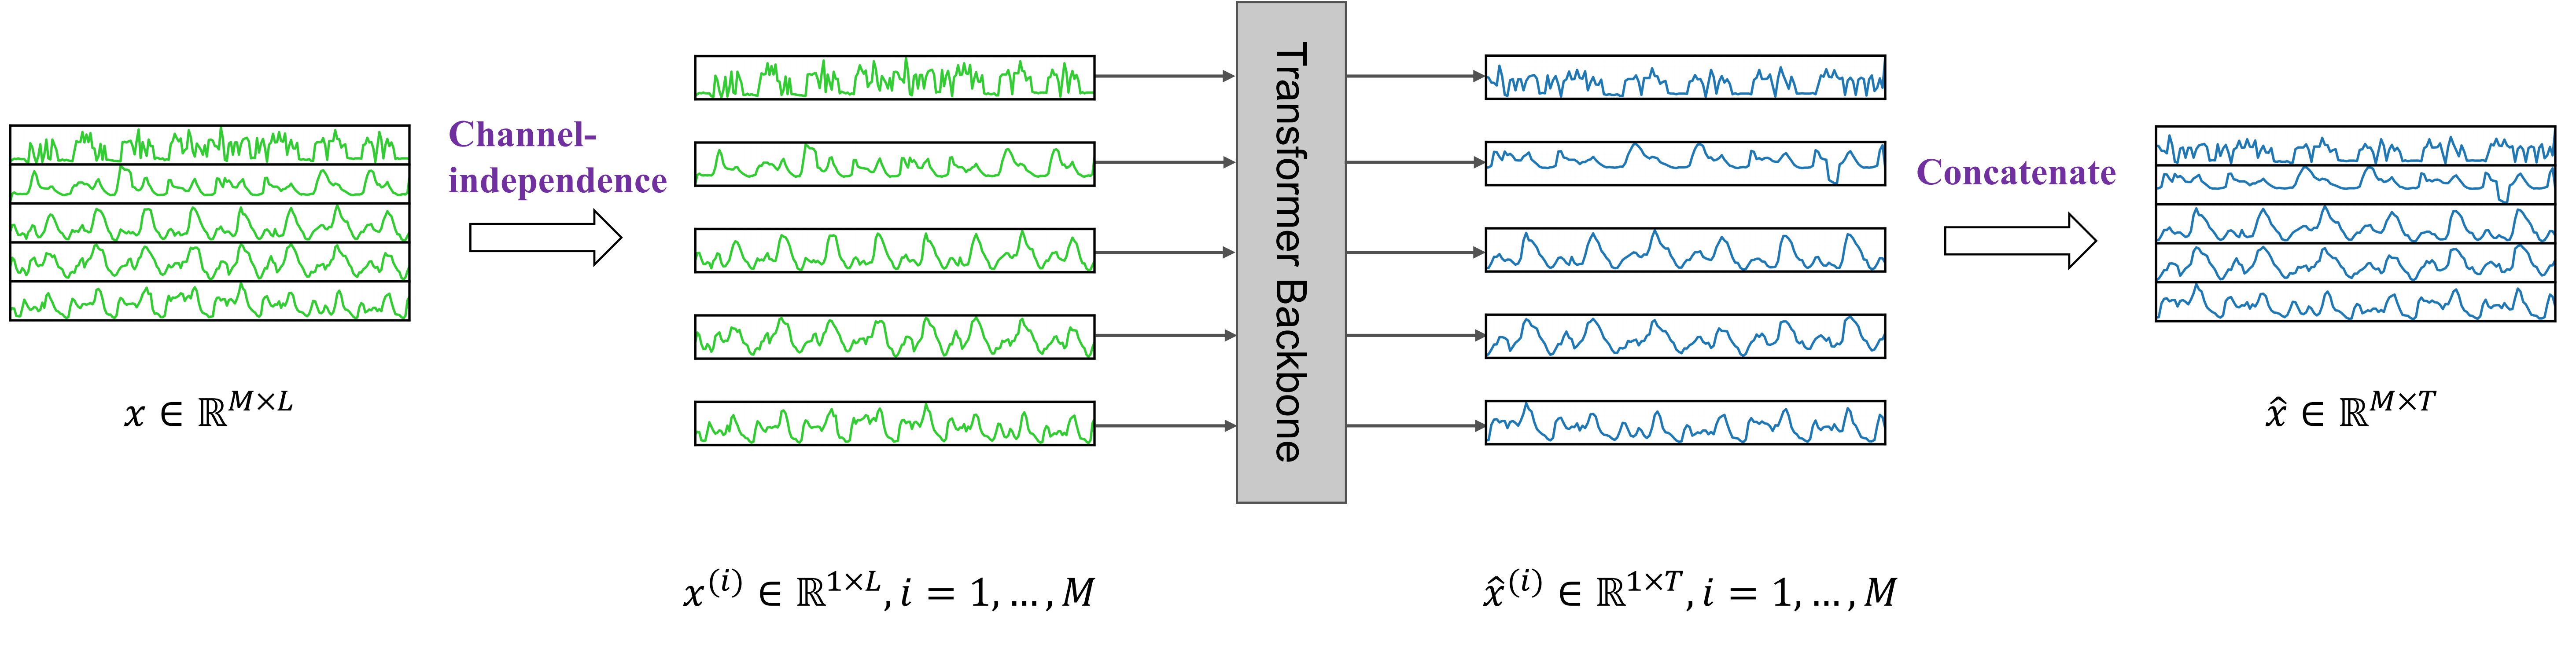
\includegraphics[width=0.5
%    \textwidth]{bibliography/Figure/patchTST(a).png}
%        \caption{(a) Tổng quan mô hình PatchTST}
%        \label{fig:example}
%    \end{figure}
   
%    \begin{enumerate}
%        \item Đầu vào đa biến \( \mathbf{x} \in \mathbb{R}^{M \times L} \): Chuỗi thời gian đầu vào có \( M \) kênh (hoặc biến) và mỗi kênh có độ dài \( L \).
%        \item Độc lập kênh: Mỗi kênh \( \mathbf{x}^{(i)} \in \mathbb{R}^{1 \times L} \), với \( i = 1, \ldots, M \), được xử lý riêng biệt và độc lập.
%        \item Transformer Backbone: Mỗi chuỗi đơn biến được đưa vào Transformer Backbone riêng lẻ để tạo ra kết quả dự báo \( \hat{\mathbf{x}}^{(i)} \in \mathbb{R}^{1 \times T} \).
%        \item Ghép kênh (Concatenate): Kết quả dự báo từ các kênh độc lập được ghép lại để tạo ra dự báo đầu ra cuối cùng \( \hat{\mathbf{x}} \in \mathbb{R}^{M \times T} \).
%    \end{enumerate}
   
%    \paragraph{Backbone của Transformer (Giám sát)}
   
%    \begin{figure}[h]
%        \centering
%    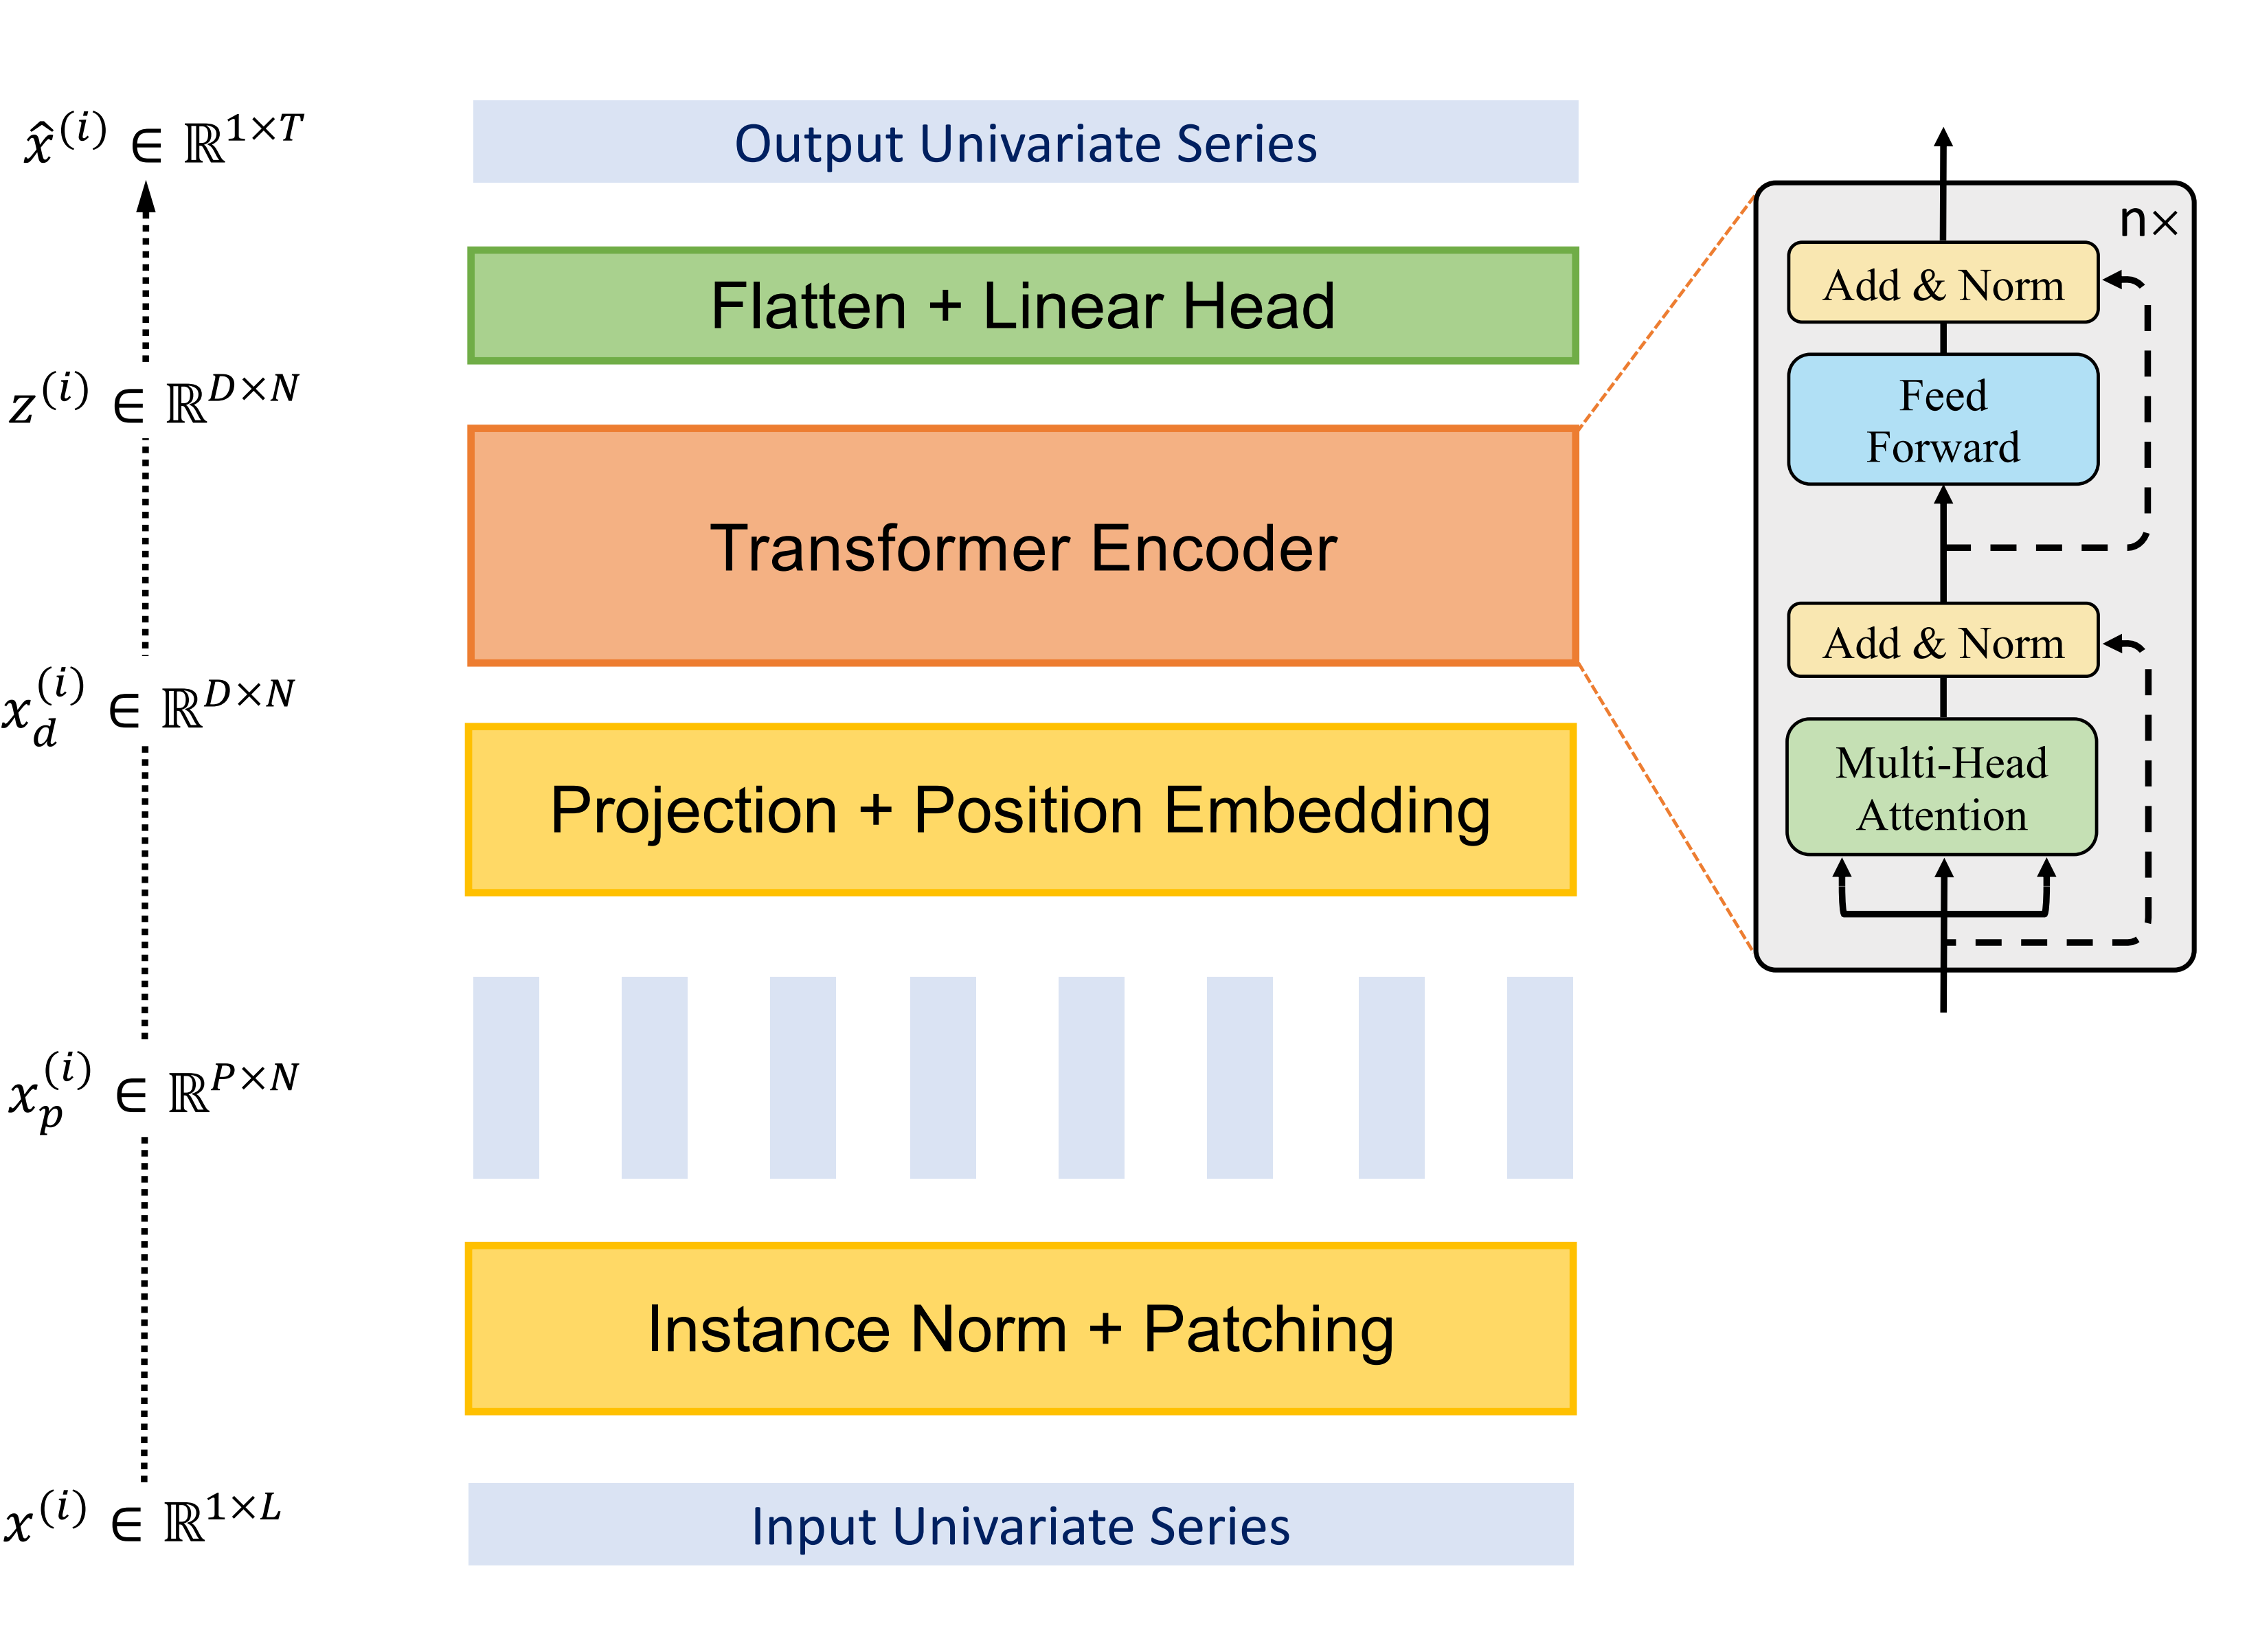
\includegraphics[width=0.4
%    \textwidth]{bibliography/Figure/patchTST (b).png}
%        \caption{Backbone của Transformer (Giám sát)}
%        \label{fig:example}
%    \end{figure}
   
%    \begin{enumerate}
%        \item Chuỗi đơn biến đầu vào: Chuỗi thời gian đơn biến \( \mathbf{x}^{(i)} \in \mathbb{R}^{1 \times L} \).
%        \item Instance Norm + Patching: Áp dụng chuẩn hóa instance và chia chuỗi thời gian thành các đoạn (patches). Mỗi đoạn có chiều dài \( P \) và khoảng cách giữa các đoạn là \( S \).
%        \item Projection + Position Embedding: Chiếu các đoạn vào không gian tiềm ẩn và thêm embedding vị trí để bảo toàn thứ tự thời gian. Công thức:
%        \[
%        \mathbf{x}^{(i)}_d = W_p \mathbf{x}^{(i)}_p + W_{\text{pos}}
%        \]
%        trong đó \( W_p \) là ma trận chiếu và \( W_{\text{pos}} \) là embedding vị trí.
%        \item Transformer Encoder: Encoder của Transformer xử lý các đoạn để tạo ra biểu diễn tiềm ẩn \( \mathbf{z}^{(i)} \in \mathbb{R}^{D \times N} \).
%        \item Flatten + Linear Head: Làm phẳng và sử dụng đầu tuyến tính để tạo ra dự báo đầu ra \( \hat{\mathbf{x}}^{(i)} \in \mathbb{R}^{1 \times T} \).
%    \end{enumerate}
   
%    \paragraph{Backbone của Transformer (Tự giám sát)}
%    \begin{figure}[h]
%        \centering
%    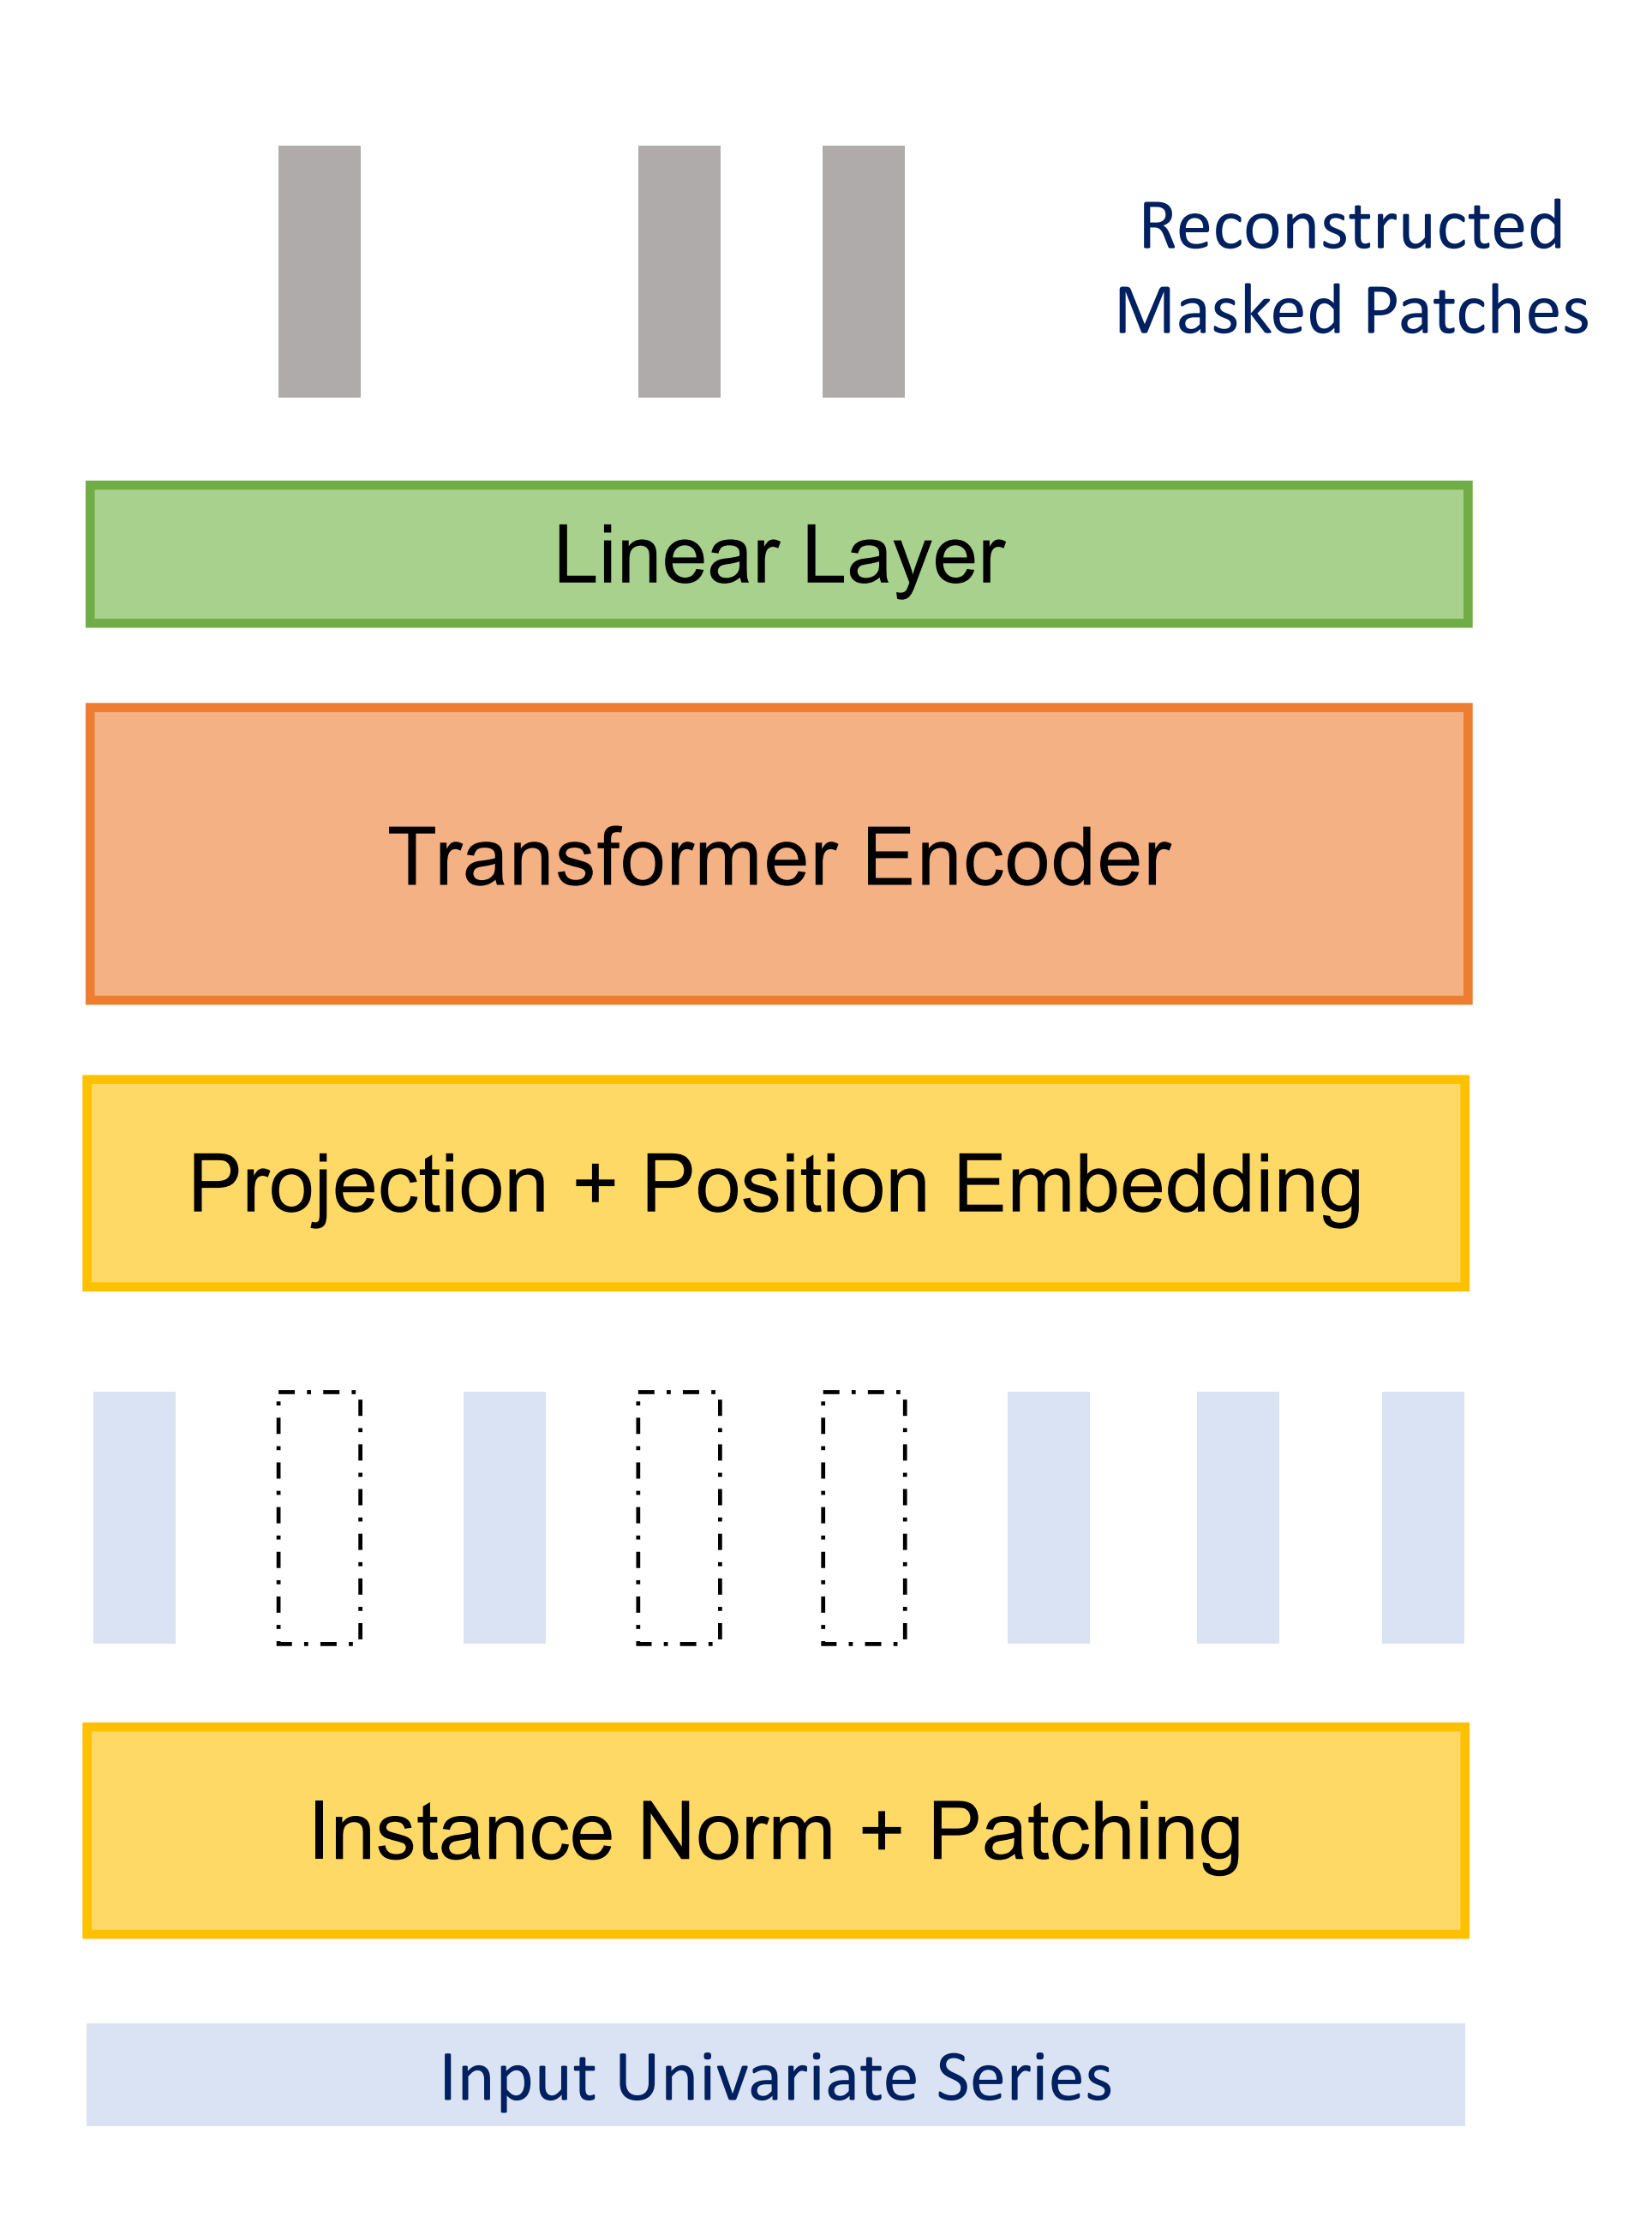
\includegraphics[width=0.3
%    \textwidth]{bibliography/Figure/patchTST(C).png}
%        \caption{Backbone của Transformer (Tự giám sát)}
%        \label{fig:example}
%    \end{figure}
   
%    \begin{enumerate}
%        \item Chuỗi đơn biến đầu vào: Tương tự như phần giám sát.
%        \item Instance Norm + Patching: Tương tự như phần giám sát, nhưng có thêm bước chọn ngẫu nhiên các đoạn để đặt giá trị bằng không (masking).
%        \item Projection + Position Embedding: Tương tự như phần giám sát.
%        \item Transformer Encoder: Tương tự như phần giám sát, nhưng với nhiệm vụ tái tạo lại các đoạn đã bị mask.
%        \item Linear Layer: Lớp tuyến tính để tái tạo lại các đoạn bị mask.
%    \end{enumerate}
   
%    \paragraph{Công thức chính}
   
%    \begin{itemize}
%        \item Patching:
%        \[
%        N = \left\lfloor \frac{L - P}{S} \right\rfloor + 1
%        \]
%        trong đó \( N \) là số lượng đoạn, \( L \) là độ dài chuỗi thời gian, \( P \) là chiều dài mỗi đoạn, và \( S \) là khoảng cách giữa các đoạn.
%        \item Projection + Position Embedding:
%        \[
%        \mathbf{x}^{(i)}_d = W_p \mathbf{x}^{(i)}_p + W_{\text{pos}}
%        \]
%        trong đó \( \mathbf{x}^{(i)}_d \) là đầu vào của Transformer encoder, \( W_p \) là ma trận chiếu, và \( W_{\text{pos}} \) là embedding vị trí.
%    \end{itemize}
   
%    Mục tiêu của PatchTST là nâng cao độ chính xác và hiệu quả trong dự đoán chuỗi thời gian dài hạn. Điểm mạnh của mô hình bao gồm khả năng xử lý hiệu quả, học các mẫu phức tạp và độ chính xác cao nhờ vào attention mechanism. Tuy nhiên, nó đòi hỏi nhiều tài nguyên tính toán và cần được tinh chỉnh cẩn thận về kích thước đoạn, đồng thời yêu cầu kiến thức chuyên môn để triển khai hiệu quả.

% \section{Thực nghiệm}
% \subsection{Các độ đo}
%         \subsubsection{Root Mean Square Error (RMSE)}
%         RMSE là kích thước trung bình của sai số tuyệt đối giữa giá trị thực tế và giá trị dự báo.
%         \[
%         \text{RMSE} = \sqrt{\frac{\sum (y - \hat{y})^2}{n}}
%         \]

%         \subsubsection{Mean Absolute Percentage Error (MAPE)}
%         MAPE là tỷ lệ phần trăm trung bình giữa sai số tuyệt đối và giá trị thực tế.
%         \[
%         \text{MAPE} = \frac{1}{n} \sum \left| \frac{y - \hat{y}}{y} \right|
%         \]

%         \subsubsection{Mean Absolute Error (MAE)}
%         MAE là trung bình của sai số tuyệt đối giữa giá trị thực tế \(y\) và giá trị dự báo \(\hat{y}\).
%         \[
%         \text{MAE} = \frac{1}{n} \sum |y - \hat{y}|
%         \]

%         \vspace{1em}
%         Ký hiệu:
%         \begin{itemize}
%             \item \( y \): giá trị thực tế của điểm dữ liệu \(x\)
%             \item \( \hat{y} \): giá trị mô hình dự đoán cho điểm dữ liệu \(x\)
%         \end{itemize}
        

%         \subsection{Dự báo}
%             \paragraph{THB\_USD} Dưới đây là dự báo và kết quả đánh giá của các mô hình được chia theo lần lượt mức chia 9:1, 8:2 và 7:3 của THB\_USD 

%                 \begin{figure}[h!]
%                     \centering
%                     \begin{minipage}{0.17\textwidth}
%                     \centering
%                     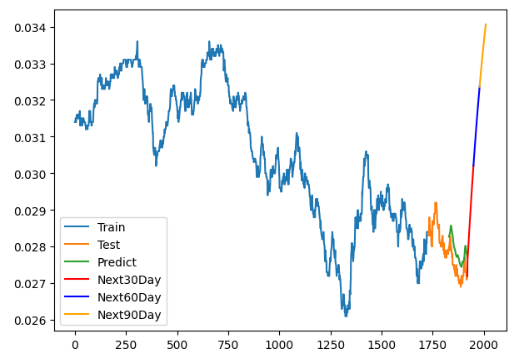
\includegraphics[width=1\textwidth]{Hình dự báo/Boosting Model/Thailan/ThaiLan_9-1.png}
                
%                     \label{fig:1}
%                     \end{minipage}%
%                     \begin{minipage}{0.17\textwidth}
%                     \centering
%                     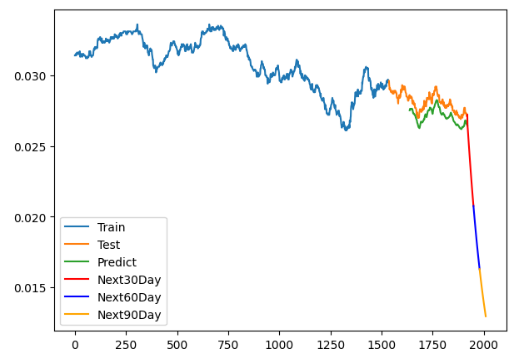
\includegraphics[width=1\textwidth]{Hình dự báo/Boosting Model/Thailan/ThaiLan_8-2.png}
                
%                     \label{fig:2}
%                     \end{minipage}%
%                     \begin{minipage}{0.17\textwidth}
%                     \centering
%                     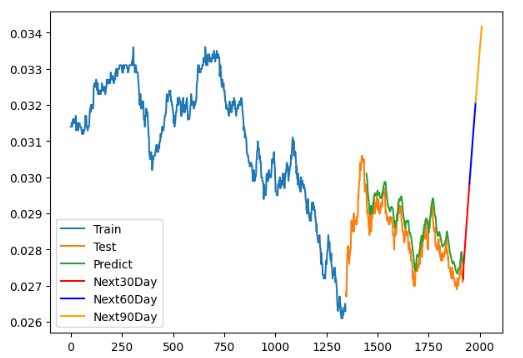
\includegraphics[width=1\textwidth]{Hình dự báo/Boosting Model/Thailan/ThaiLan_7-3.png}

%                     \label{fig:3}
%                     \end{minipage}
%                     \caption{30, 60, 90 ngày trên bộ dữ liệu THB\_USD của mô hình GRU}
%                 \end{figure}

%                 \begin{figure}[h!]
%                     \centering
%                     \begin{minipage}{0.17\textwidth}
%                     \centering
%                     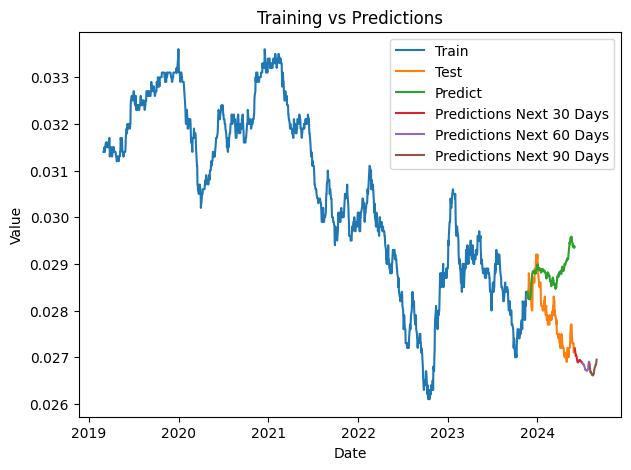
\includegraphics[width=1\textwidth]{Hình dự báo/PatchTST/THB_USD/PatchTST_THB_USD_91.png}
                
%                     \label{fig:1}
%                     \end{minipage}%
%                     \begin{minipage}{0.17\textwidth}
%                     \centering
%                     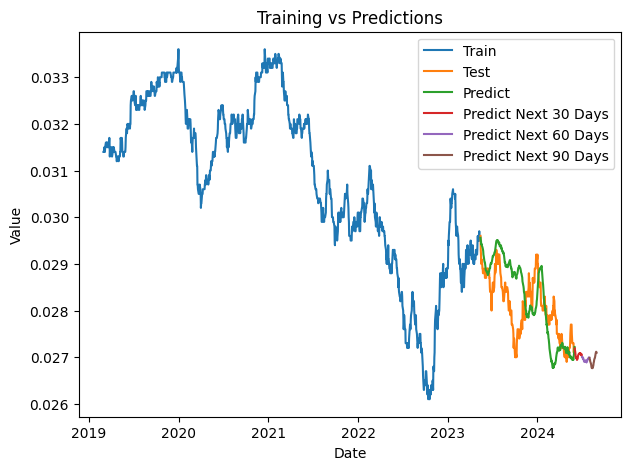
\includegraphics[width=1\textwidth]{Hình dự báo/PatchTST/THB_USD/PatchTST_THB_USD_82.png}
                
%                     \label{fig:2}
%                     \end{minipage}%
%                     \begin{minipage}{0.17\textwidth}
%                     \centering
%                     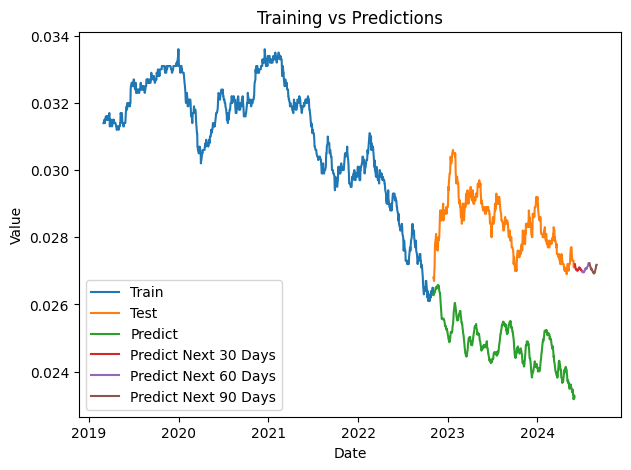
\includegraphics[width=1\textwidth]{Hình dự báo/PatchTST/THB_USD/PatchTST_THB_USD_73.png}

%                     \label{fig:3}
%                     \end{minipage}
%                     \caption{30, 60, 90 ngày trên bộ dữ liệu THB\_USD của mô hình PatchTST}
%                 \end{figure}
%                 \FloatBarrier

%                 \FloatBarrier
%                 \begin{table}[h!]
%                     \centering
%                     \begin{tabular}{|l|l|c|c|c|}
%                     \hline
%                     \multirow{2}{*}{\textbf{Model}} & \multirow{2}{*}{\textbf{Metric}} & \multicolumn{3}{c|}{\textbf{THB\_USD}} \\ \cline{3-5} 
%                      &  & \textbf{9-1} & \textbf{8-2} & \textbf{7-3} \\ \hline
%                     \multirow{3}{*}{\textbf{Linear Regression}} & RMSE & 0.0005 & 0.0005 & 0.0009 \\ \cline{2-5} 
%                      & MAE & \textcolor{red}{\textbf{0.0004}} & \textcolor{red}{\textbf{0.0004}} & 0.0007 \\ \cline{2-5} 
%                      & MAPE & \textcolor{red}{\textbf{0.0148}} & \textcolor{red}{\textbf{0.0154}} & 0.0254 \\ \hline
%                     \multirow{3}{*}{\textbf{ARIMA}} & RMSE & 0.0008 & 0.0016 & 0.0033 \\ \cline{2-5} 
%                      & MAE & 0.0007 & 0.0015 & 0.0032 \\ \cline{2-5} 
%                      & MAPE & 0.0235 & 0.0498 & 0.1283 \\ \hline
%                     \multirow{3}{*}{\textbf{RNN}} & RMSE & 0.0197 & 0.0171 & 0.0211 \\ \cline{2-5} 
%                      & MAE & 0.0156 & 0.0128 & 0.0163 \\ \cline{2-5} 
%                      & MAPE & 0.0774 & 0.0545 & 0.0601 \\ \hline
%                     \multirow{3}{*}{\textbf{GRU}} & RMSE & 0.0005 & 0.0008 & 0.001 \\ \cline{2-5} 
%                      & MAE & \textcolor{red}{\textbf{0.0004}} & 0.0007 & 0.0008 \\ \cline{2-5} 
%                      & MAPE & 1.549 & 2.456 & 2.9207 \\ \hline
%                     \multirow{3}{*}{\textbf{LSTM}} & RMSE & 0.1557 & 0.2208 & 0.2816 \\ \cline{2-5} 
%                      & MAE & 0.1488 & 0.2085 & 0.2654 \\ \cline{2-5} 
%                      & MAPE & 5.3898 & 7.4272 & 9.3216 \\ \hline
%                     \multirow{3}{*}{\textbf{FFT}} & RMSE & 0.0016 & 0.0011 & 0.0014 \\ \cline{2-5} 
%                      & MAE & 0.0013 & 0.0009 & 0.0011 \\ \cline{2-5} 
%                      & MAPE & 4.5357 & 3.0747 & 3.8007 \\ \hline
%                     \multirow{3}{*}{\textbf{PatchTST}} & RMSE & 0.0012 & 0.0007 & 0.0037 \\ \cline{2-5} 
%                      & MAE & 0.0010 & 0.0005 & 0.0036 \\ \cline{2-5} 
%                      & MAPE & 0.0368 & 0.0204 & 0.1262 \\ \hline
%                     \multirow{3}{*}{\textbf{FEDformer}} & RMSE & 0.0025 & 0.0011 & 0.0006 \\ \cline{2-5} 
%                      & MAE & 6.3735 & 1.1513 & 3.6430 \\ \cline{2-5} 
%                      & MAPE & 0.0839 & 0.0334 & \textcolor{red}{\textbf{0.0173}} \\ \hline
%                     \multirow{3}{*}{\textbf{Boosting Model}} & RMSE & \textcolor{red}{\textbf{0.0001}} & \textcolor{red}{\textbf{0.0001}} & \textcolor{red}{\textbf{0.0005}} \\ \cline{2-5} 
%                      & MAE & 0.3248 & 0.3401 & \textcolor{red}{\textbf{0.0004}} \\ \cline{2-5} 
%                      & MAPE & 8.8951 & 9.4617 & 1.3621 \\ \hline
%                     \multirow{3}{*}{\textbf{TBATS}} & RMSE & 0.0011 & 0.0016 & 0.0018 \\ \cline{2-5} 
%                      & MAE & 0.001 & 0.0014 & 0.0016 \\ \cline{2-5} 
%                      & MAPE & 0.0339 & 0.048 & 0.0581 \\ \hline
%                     \end{tabular}
%                     \caption{Kết quả đánh giá của THB\_USD}
%                     \label{tab:forecasting_results_thb}
%                 \end{table}
%                 \FloatBarrier


% \paragraph{MXN\_USD} Dưới đây là dự báo và kết quả đánh giá của các mô hình được chia theo lần lượt mức chia 9:1, 8:2 và 7:3 của MXN\_USD 

% \begin{figure}[h!]
%     \centering
%     \begin{minipage}{0.17\textwidth}
%     \centering
%     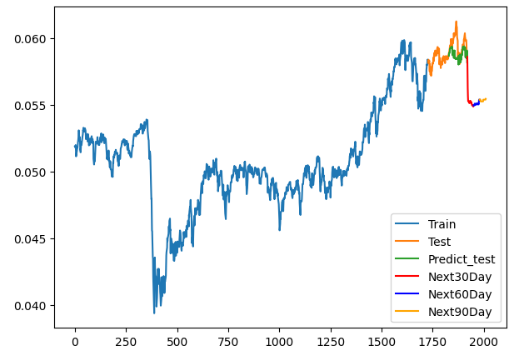
\includegraphics[width=1\textwidth]{Hình dự báo/Boosting Model/Mexico/MXC_9-1.png}
   
%     \label{fig:1}
%     \end{minipage}%
%     \begin{minipage}{0.17\textwidth}
%     \centering
%     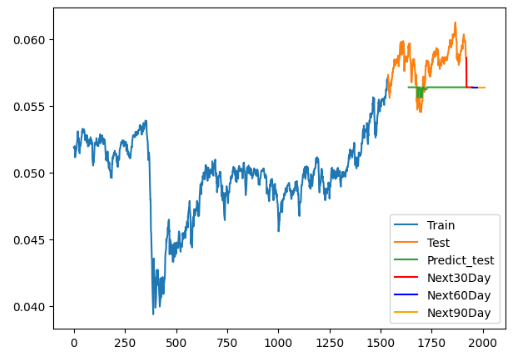
\includegraphics[width=1\textwidth]{Hình dự báo/Boosting Model/Mexico/MXC_8-2.png}
  
%     \label{fig:2}
%     \end{minipage}%
%     \begin{minipage}{0.17\textwidth}
%     \centering
%     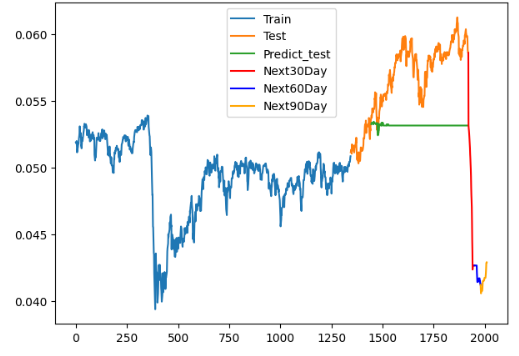
\includegraphics[width=1\textwidth]{Hình dự báo/Boosting Model/Mexico/MXC_7-3.png}

%     \label{fig:3}
%     \end{minipage}
%     \caption{30, 60, 90 ngày trên bộ dữ liệu MXN\_USD của mô hình Boosting Model }
% \end{figure}

% \begin{figure}[h!]
%     \centering
%     \begin{minipage}{0.17\textwidth}
%     \centering
%     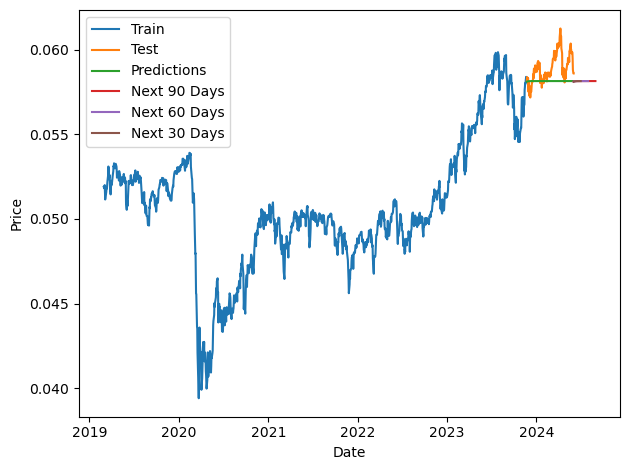
\includegraphics[width=1\textwidth]{Hình dự báo/TBATS/MXN_USD/TBATS 91.png}
   
%     \label{fig:1}
%     \end{minipage}%
%     \begin{minipage}{0.17\textwidth}
%     \centering
%     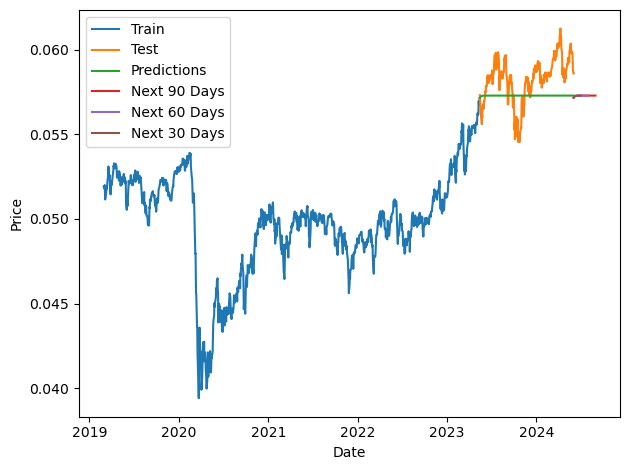
\includegraphics[width=1\textwidth]{Hình dự báo/TBATS/MXN_USD/TBATS 82.png}
  
%     \label{fig:2}
%     \end{minipage}%
%     \begin{minipage}{0.17\textwidth}
%     \centering
%     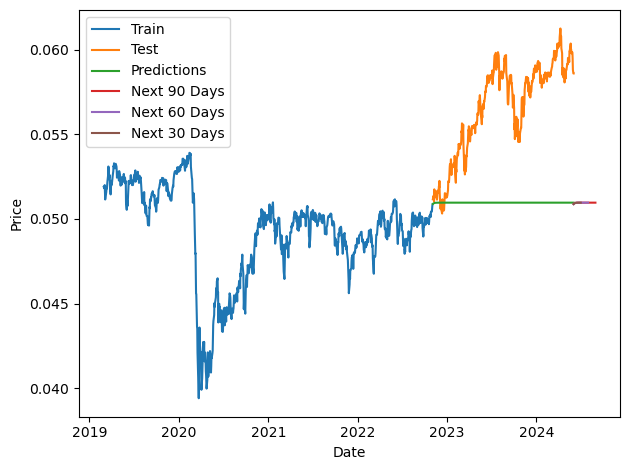
\includegraphics[width=1\textwidth]{Hình dự báo/TBATS/MXN_USD/TBATS 73.png}

%     \label{fig:3}
%     \end{minipage}
%     \caption{30, 60, 90 ngày trên bộ dữ liệu MXN\_USD của mô hình TBATS}
% \end{figure}

% \FloatBarrier
% \begin{table}[h!]
%     \centering
%     \begin{tabular}{|l|l|c|c|c|}
%     \hline
%     \multirow{2}{*}{\textbf{Model}} & \multirow{2}{*}{\textbf{Metric}} & \multicolumn{3}{c|}{\textbf{MXN\_USD}} \\ \cline{3-5} 
%      &  & \textbf{9-1} & \textbf{8-2} & \textbf{7-3} \\ \hline
%     \multirow{3}{*}{\textbf{Linear Regression}} & RMSE & 0.0051 & 0.0077 & 0.0091 \\ \cline{2-5} 
%      & MAE & 0.0051 & 0.0076 & 0.0086 \\ \cline{2-5} 
%      & MAPE & 0.0942 & 0.1495 & 0.1784 \\ \hline
%     \multirow{3}{*}{\textbf{ARIMA}} & RMSE & 0.0012 & 0.0017 & 0.0064 \\ \cline{2-5} 
%      & MAE & 0.0009 & 0.0015 & 0.0057 \\ \cline{2-5} 
%      & MAPE & 0.0161 & 0.0263 & 0.1132 \\ \hline
%     \multirow{3}{*}{\textbf{RNN}} & RMSE & 0.0167 & 0.0341 & 0.0165 \\ \cline{2-5} 
%      & MAE & 0.0133 & 0.0318 & 0.0133 \\ \cline{2-5} 
%      & MAPE & \textcolor{red}{\textbf{0.0151}} & 0.0365 & \textcolor{red}{\textbf{0.0171}} \\ \hline
%     \multirow{3}{*}{\textbf{GRU}} & RMSE & 0.0013 & 0.0019 & \textcolor{red}{\textbf{0.0026}} \\ \cline{2-5} 
%      & MAE & 0.0011 & 0.0015 & \textcolor{red}{\textbf{0.002}} \\ \cline{2-5} 
%      & MAPE & 1.773 & 2.603 & 3.517 \\ \hline
%     \multirow{3}{*}{\textbf{LSTM}} & RMSE & 0.8629 & 0.8087 & 0.7807 \\ \cline{2-5} 
%      & MAE & 0.8623 & 0.8061 & 0.7762 \\ \cline{2-5} 
%      & MAPE & 14.5718 & 13.7032 & 13.462 \\ \hline
%     \multirow{3}{*}{\textbf{FFT}} & RMSE & 0.0017 & 0.0051 & 0.0107 \\ \cline{2-5} 
%      & MAE & 0.0013 & 0.0048 & 0.0089 \\ \cline{2-5} 
%      & MAPE & 2.2130 & 8.1531 & 15.2636 \\ \hline
%     \multirow{3}{*}{\textbf{PatchTST}} & RMSE & 0.0013 & 0.0023 & 0.0073 \\ \cline{2-5} 
%      & MAE & 0.0010 & 0.0020 & 0.0068 \\ \cline{2-5} 
%      & MAPE & 0.0168 & 0.0339 & 0.1175 \\ \hline
%     \multirow{3}{*}{\textbf{FEDformer}} & RMSE & 0.0041 & 0.0037 & 0.0077 \\ \cline{2-5} 
%      & MAE & 1.6658 & 1.3466 & 5.8668 \\ \cline{2-5} 
%      & MAPE & 0.0672 & 0.0579 & 0.1237 \\ \hline
%     \multirow{3}{*}{\textbf{Boosting Model}} & RMSE & \textcolor{red}{\textbf{0.0008}} & 0.0021 & 0.0048 \\ \cline{2-5} 
%      & MAE & \textcolor{red}{\textbf{0.0006}} & 0.0019 & 0.0044 \\ \cline{2-5} 
%      & MAPE & 1.0074 & 3.2561 & 7.5973 \\ \hline
%     \multirow{3}{*}{\textbf{TBATS}} & RMSE & 0.0011 & \textcolor{red}{\textbf{0.0016}} & 0.0063 \\ \cline{2-5} 
%      & MAE & 0.0009 & \textcolor{red}{\textbf{0.0014}} & 0.0057 \\ \cline{2-5} 
%      & MAPE & 0.0152 & \textcolor{red}{\textbf{0.0251}} & 0.1116 \\ \hline
%     \end{tabular}
%     \caption{Kết quả đánh giá của MXN\_USD}
%     \label{tab:forecasting_results_mxn}
% \end{table}
% \FloatBarrier


% \paragraph{JPY\_USD} Dưới đây là dự báo và kết quả đánh giá của các mô hình được chia theo lần lượt mức chia 9:1, 8:2 và 7:3 của JPY\_USD 

% \begin{figure}[h!]
%     \centering
%     \begin{minipage}{0.17\textwidth}
%     \centering
%     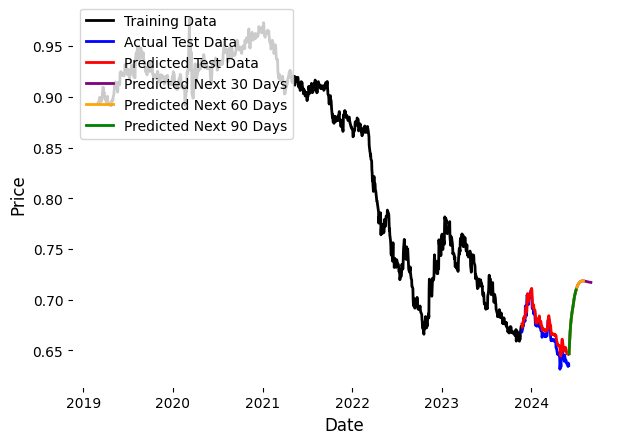
\includegraphics[width=1\textwidth]{Hình dự báo/RNN/JPY_USD/RNN_JPY_USD_91.png}
   
%     \label{fig:1}
%     \end{minipage}%
%     \begin{minipage}{0.17\textwidth}
%     \centering
%     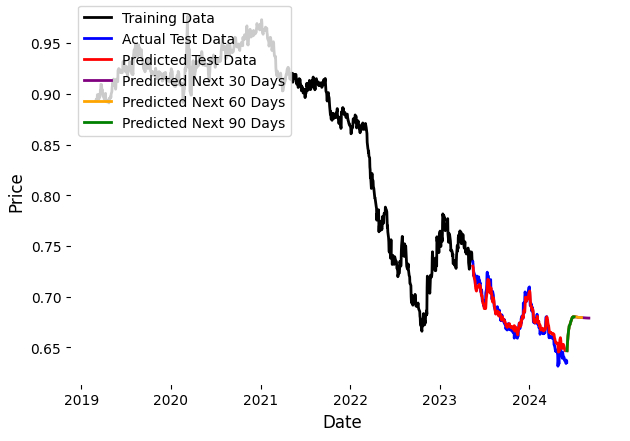
\includegraphics[width=1\textwidth]{Hình dự báo/RNN/JPY_USD/RNN_JPY_USD_82.png}
  
%     \label{fig:2}
%     \end{minipage}%
%     \begin{minipage}{0.17\textwidth}
%     \centering
%     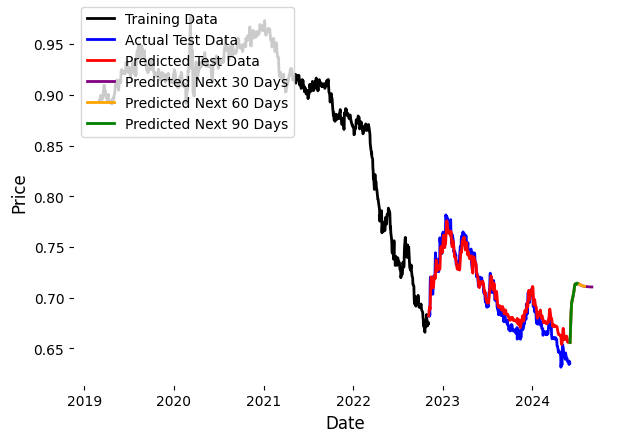
\includegraphics[width=1\textwidth]{Hình dự báo/RNN/JPY_USD/RNN_JPY_USD_73.png}

%     \label{fig:3}
%     \end{minipage}
%     \caption{30, 60, 90 ngày trên bộ dữ liệu JPY\_USD của mô hình RNN}
% \end{figure}

% \begin{figure}[h!]
%     \centering
%     \begin{minipage}{0.17\textwidth}
%     \centering
%     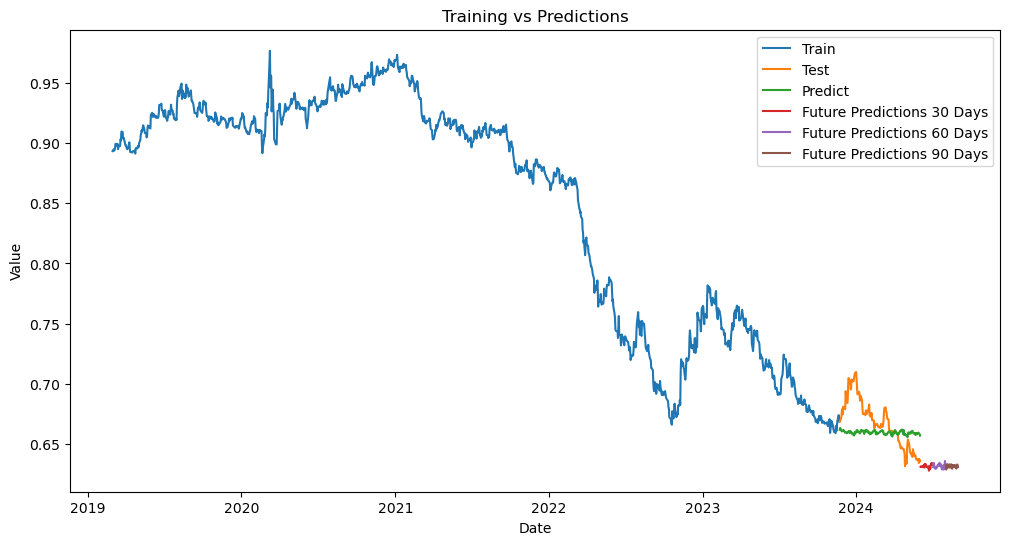
\includegraphics[width=1\textwidth]{Hình dự báo/FEDformer/JPY_USD_9-1.png}
   
%     \label{fig:1}
%     \end{minipage}%
%     \begin{minipage}{0.17\textwidth}
%     \centering
%     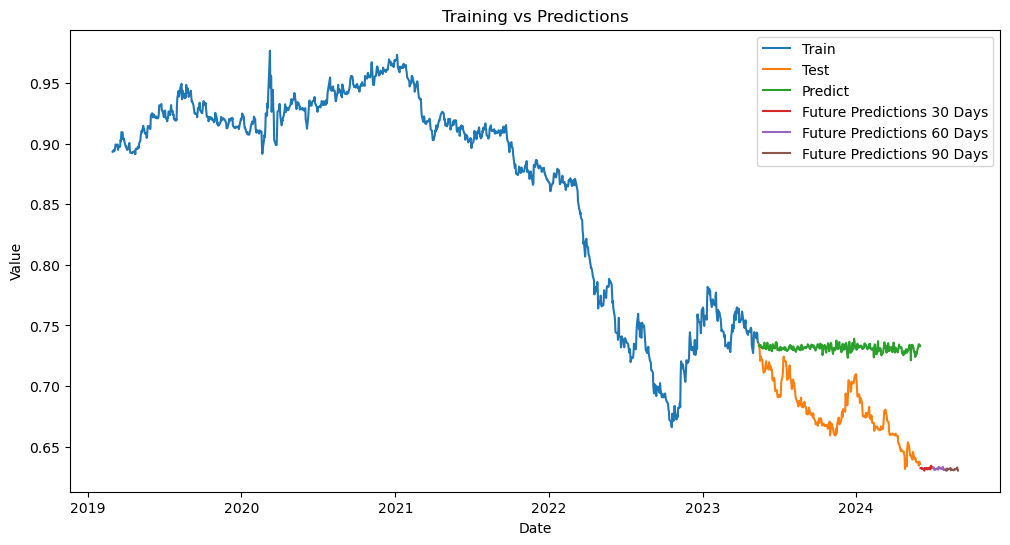
\includegraphics[width=1\textwidth]{Hình dự báo/FEDformer/JPY_USD_8-2.png}
  
%     \label{fig:2}
%     \end{minipage}%
%     \begin{minipage}{0.17\textwidth}
%     \centering
%     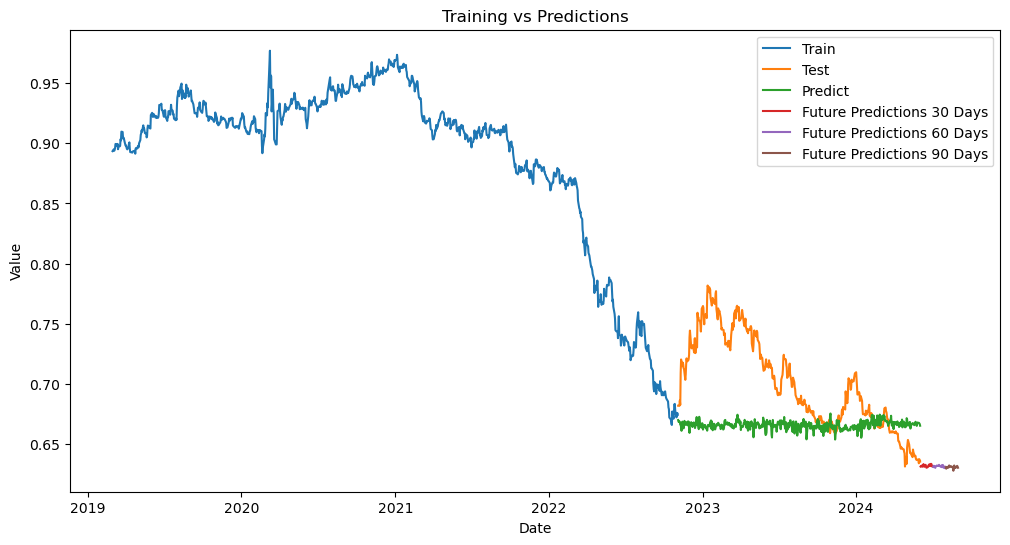
\includegraphics[width=1\textwidth]{Hình dự báo/FEDformer/JPY_USD_7-3.png}

%     \label{fig:3}
%     \end{minipage}
%     \caption{30, 60, 90 ngày trên bộ dữ liệu JPY\_USD của mô hình FEDFormer}
% \end{figure}

% \FloatBarrier
% \begin{table}[h!]
%     \centering
%     \begin{tabular}{|l|l|c|c|c|}
%     \hline
%     \multirow{2}{*}{\textbf{Model}} & \multirow{2}{*}{\textbf{Metric}} & \multicolumn{3}{c|}{\textbf{JPY\_USD}} \\ \cline{3-5} 
%      &  & \textbf{9-1} & \textbf{8-2} & \textbf{7-3} \\ \hline
%     \multirow{3}{*}{\textbf{Linear Regression}} & RMSE & 0.0249 & 0.0496 & 0.0645 \\ \cline{2-5} 
%      & MAE & 0.0224 & 0.0476 & 0.0608 \\ \cline{2-5} 
%      & MAPE & 0.0326 & \textcolor{red}{\textbf{0.0656}} & 0.0803 \\ \hline
%     \multirow{3}{*}{\textbf{ARIMA}} & RMSE & 0.0185 & 0.0608 & 0.2033 \\ \cline{2-5} 
%      & MAE & 0.0145 & 0.0564 & 0.1923 \\ \cline{2-5} 
%      & MAPE & \textcolor{red}{\textbf{0.022}} & 0.0767 & 0.4175 \\ \hline
%     \multirow{3}{*}{\textbf{RNN}} & RMSE & \textcolor{red}{\textbf{0.0175}} & \textcolor{red}{\textbf{0.0124}} & 0.0278 \\ \cline{2-5} 
%      & MAE & 0.0205 & 0.0161 & 0.0226 \\ \cline{2-5} 
%      & MAPE & 1412 & 7019 & 6723 \\ \hline
%     \multirow{3}{*}{\textbf{GRU}} & RMSE & 0.0179 & 0.0236 & 0.0477 \\ \cline{2-5} 
%      & MAE & 0.014 & 0.0186 & 0.0382 \\ \cline{2-5} 
%      & MAPE & 2.197 & 2.778 & 5.494 \\ \hline
%     \multirow{3}{*}{\textbf{LSTM}} & RMSE & 0.5968 & 0.567 & 0.5267 \\ \cline{2-5} 
%      & MAE & 0.5955 & 0.5647 & 0.5167 \\ \cline{2-5} 
%      & MAPE & 0.9073 & 0.8389 & 0.7526 \\ \hline
%     \multirow{3}{*}{\textbf{FFT}} & RMSE & 0.0601 & 0.0361 & 0.0650 \\ \cline{2-5} 
%      & MAE & 0.0501 & 0.0298 & 0.0539 \\ \cline{2-5} 
%      & MAPE & 7.3663 & 4.4068 & 7.9436 \\ \hline
%     \multirow{3}{*}{\textbf{PatchTST}} & RMSE & 0.0203 & 0.0591 & 0.0649 \\ \cline{2-5} 
%      & MAE & 0.0163 & 0.0536 & 0.0525 \\ \cline{2-5} 
%      & MAPE & 0.0241 & 0.0802 & 0.0726 \\ \hline
%     \multirow{3}{*}{\textbf{FEDformer}} & RMSE & 0.0516 & 0.0570 & 0.0214 \\ \cline{2-5} 
%      & MAE & \textcolor{red}{\textbf{0.0027}} & \textcolor{red}{\textbf{0.0032}} & \textcolor{red}{\textbf{0.0004}} \\ \cline{2-5} 
%      & MAPE & 0.0556 & 0.0784 & \textcolor{red}{\textbf{0.0255}} \\ \hline
%     \multirow{3}{*}{\textbf{Boosting Model}} & RMSE & 0.0215 & 0.0373 & \textcolor{red}{\textbf{0.0179}} \\ \cline{2-5} 
%      & MAE & 0.0185 & 0.0344 & 0.0143 \\ \cline{2-5} 
%      & MAPE & 2.8677 & 5.2064 & 2.0828 \\ \hline
%     \multirow{3}{*}{\textbf{TBATS}} & RMSE & 0.0199 & 0.065 & 0.0471 \\ \cline{2-5} 
%      & MAE & 0.0163 & 0.0609 & 0.0364 \\ \cline{2-5} 
%      & MAPE & 0.0243 & 0.0823 & 0.0541 \\ \hline
%     \end{tabular}
%     \break
%     \caption{Kết quả đánh giá của JPY\_USD}
%     \label{tab:forecasting_results_jpy}
% \end{table}
% \FloatBarrier

% \section{Kết luận}
% \begin{itemize}
%     \item \textbf{Hiệu suất của các mô hình}:
%     \begin{itemize}
%         \item \textbf{RNN} và \textbf{GRU} cho thấy hiệu suất ổn định với các giá trị RMSE, MAE và MAPE khá thấp, đặc biệt là GRU khi so sánh với các mô hình khác.
%         \item \textbf{LSTM} có hiệu suất kém hơn so với RNN và GRU, đặc biệt là về các chỉ số RMSE và MAE.
%         \item \textbf{FFT} và \textbf{PatchTST} cung cấp kết quả tốt với các chỉ số MAE và MAPE thấp, tuy nhiên FFT có lợi thế về tốc độ xử lý.
%         \item \textbf{Boosting Model} cũng cho thấy tiềm năng cao trong việc dự báo tỷ giá với các chỉ số lỗi thấp, đặc biệt là Boosting Model.
%         \item \textbf{TBATS} cung cấp kết quả tốt nhưng không nổi bật so với các mô hình học sâu.
%     \end{itemize}
%     \item \textbf{Tính ứng dụng}:
%     \begin{itemize}
%         \item Các mô hình học sâu như GRU và RNN có khả năng nắm bắt các phụ thuộc phức tạp theo thời gian trong dữ liệu, phù hợp với các dự báo ngắn hạn và dài hạn.
%         \item FFT có lợi thế về hiệu quả và tốc độ, phù hợp với các ứng dụng yêu cầu xử lý nhanh chóng.
%     \end{itemize}
% \end{itemize}

% \section{Hướng phát triển}

% Để nâng cao hiệu suất và tính ứng dụng của các mô hình dự báo tỷ giá hối đoái, chúng ta có thể xem xét các hướng phát triển sau:

% \begin{itemize}
%     \item \textbf{Tích hợp mô hình lai}: Ngoài Boosting Model, kết hợp thêm các mô hình có hiệu suất tốt để tạo ra các mô hình lai, giúp tăng cường độ chính xác và giảm thiểu lỗi dự báo.
%     \item \textbf{Tối ưu hóa tham số}: Áp dụng các kỹ thuật tối ưu hóa tham số, chẳng hạn như Grid Search hoặc Bayesian Optimization, để tìm kiếm các tham số tốt nhất cho từng mô hình.
%     \item \textbf{Nâng cao dữ liệu đầu vào}: Thu thập thêm các dữ liệu liên quan, bao gồm các chỉ số kinh tế vĩ mô và các yếu tố chính trị có thể ảnh hưởng đến tỷ giá hối đoái, để cải thiện độ chính xác của dự báo.
%     \item \textbf{Phân tích độ nhạy cảm}: Thực hiện phân tích độ nhạy cảm để hiểu rõ hơn về các yếu tố ảnh hưởng mạnh đến dự báo, từ đó điều chỉnh mô hình phù hợp hơn.
% \end{itemize}

% \begin{thebibliography}{9}
%     \bibitem{b1} Aghistina Kartikadewi, Lina Audina Abdul Rosyid, Anggraeni Eka Putri, ``Prediksi Nilai Tukar Mata Uang dengan Menggunakan Metode Regresi Linear Berganda'', Jurnal Teknologi Informasi, 2020.
%     \bibitem{b2} S. F. N. Islam, A. Sholahuddin, A. S. Abdullah, ``Forecasting and Analyzing USD-IDR Exchange Rate Using XGBoost Model'', International Journal of Business and Applied Social Science, 2021.
%     \bibitem{b3} M.S. Islam, E. Hossain, ``GRU-LSTM Hybrid Model for Forex Market Prediction'', Journal of Advanced Research in Dynamical and Control Systems, 2021.
%     \bibitem{b4} Yunze Tao, Xia Sheng, ``High-Accuracy Prediction Model of EUR-USD Exchange Rate Based on RNN'', International Journal of Computational Intelligence Systems, 2023.
%     \bibitem{b5} Tian Zhou, Ziqing Ma, Qingsong Wen, Xue Wang, Liang Sun, Rong Jin, ``FEDformer: Frequency Enhanced Decomposed Transformer for Long-term Series Forecasting''.
%     \bibitem{b6} Liam Hebert, Lukasz Golab, Pascal Poupart, Robin Cohen, ``FedFormer: Contextual Federation with Attention in Reinforcement Learning''.
%     \bibitem{b7} Jaenisch, H. M., \& Handley, J. W. (n.d.). Performance Comparison of the Prophecy (Forecasting) Algorithm in FFT Form for Unseen Feature and Time-Series Prediction. Licht Strahl Engineering INC.
%     \bibitem{b8} Nie, Y., Nguyen, N. H., Sinthong, P., \& Kalagnanam, J. (2023). ``A Time Series is Worth 64 Words: Long-term Forecasting with Transformers''. ICLR 2023. arXiv:2211.14730v2 [cs.LG]
%     \bibitem{b9} De Brouwer, E., Arany, A., Simm, J., \& Moreau, Y. (2019). ``GRU-ODE-Bayes: Continuous modeling of sporadically-observed time series''. arXiv:1905.12374v2 [cs.LG]
%     \bibitem{b10} Li, H., Li, X., Hu, P., Lei, Y., Li, C., Zhou, Y., … \& Zhou, Y. (2023). ``Boosting Multi-modal Model Performance with Adaptive Gradient Modulation''. arXiv preprint arXiv:2308.07686.
% \end{thebibliography}

\end{document}
